\documentclass[../DoAn.tex]{subfiles}
\begin{document}


\section{Tổng quan kiến trúc hệ thống}


Khác với các ứng dụng web truyền thống, hệ thống ứng dụng vay và cho vay phi tập trung này được xây dựng theo mô hình ba thành phần chính: frontend, smart contract và backend, được thể hiện chi tiết bằng hình~\ref{fig:system_architecture}. Mỗi thành phần đảm nhiệm một vai trò riêng biệt, trong đó smart contract đóng vai trò trung tâm thay vì backend như trong mô hình Web2 thông thường.

Đầu tiên là frontend, đây là thành phần giao diện người dùng, chịu trách nhiệm hiển thị dữ liệu và tiếp nhận tương tác từ người dùng. Frontend không kết nối trực tiếp với blockchain mà thông qua hai kênh trung gian: Thứ nhất, thông qua Wallet Provider (MetaMask) bằng giao thức EIP-1193 (window.ethereum), khi người dùng cần ký và gửi giao dịch, frontend gọi MetaMask để yêu cầu chữ ký, MetaMask ký giao dịch và broadcast lên mạng thông qua RPC Provider (Alchemy / Infura) bằng JSON-RPC; Thứ hai, frontend đọc dữ liệu trực tiếp từ blockchain thông qua RPC Provider bằng eth\_call để lấy trạng thái real-time của các smart contracts mà không cần ký giao dịch. Ngoài ra, frontend giao tiếp với backend qua HTTPS (REST API) và nhận thông báo real-time qua WebSocket.

Tiếp theo là smart contracts, smart contract là trái tim của toàn hệ thống, đóng vai trò tương đương với backend trong mô hình Web2 truyền thống. Toàn bộ trạng thái của hệ thống bao gồm số dư tài sản, khoản vay, tỉ lệ lãi suất, và các tham số rủi ro đều được lưu trữ trên blockchain thông qua các smart contracts. Đây cũng là tầng chứa và có nhiệm vụ thực thi toàn bộ logic nghiệp vụ của hệ thống. Ngoài ra, mỗi khi có tương tác với giao thức, smart contracts sẽ phát ra các sự kiện (events) kèm theo thông tin chi tiết về hành động đó, phục vụ cho việc index dữ liệu ở tầng backend.

Cuối cùng là tầng backend, khác với mô hình Web2 nơi backend là nơi xử lý logic nghiệp vụ, backend trong hệ thống này không có quyền thay đổi trạng thái giao thức. Mục đích chính của backend đóng vai trò indexer trung gian, lưu trữ dữ liệu không thể query on-chain như lịch sử sự kiện hay dữ liệu tổng hợp, giúp người dùng theo dõi quá trình tương tác với giao thức. Backend thực hiện điều này bằng cách liên tục polling RPC Provider thông qua eth\_getLogs để lắng nghe các sự kiện mà smart contracts phát ra, sau đó xử lý dữ liệu từ sự kiện và lưu vào PostgreSQL. Bên cạnh đó, backend thực hiện snapshot hằng ngày các thông tin về tài sản giao thức và vị thế người dùng phục vụ cho việc theo dõi lịch sử. Để phối hợp giữa các tiến trình nội bộ (indexer, snapshot, notification), backend sử dụng RabbitMQ làm message broker~\cite{RabbitMQDocs} và Redis để đảm nhiệm hai vai trò: lưu trữ các dữ liệu tồn tại ngắn hạn mà không có nhu cầu phải lưu trữ database, và pub/sub để hỗ trợ WebSocket real-time đẩy thông báo tới frontend. Ngoài ra, backend cho phép người dùng đăng ký email và gửi thông báo về các thay đổi quan trọng của giao thức thông qua SMTP Service.

\begin{figure}[H]
\centering
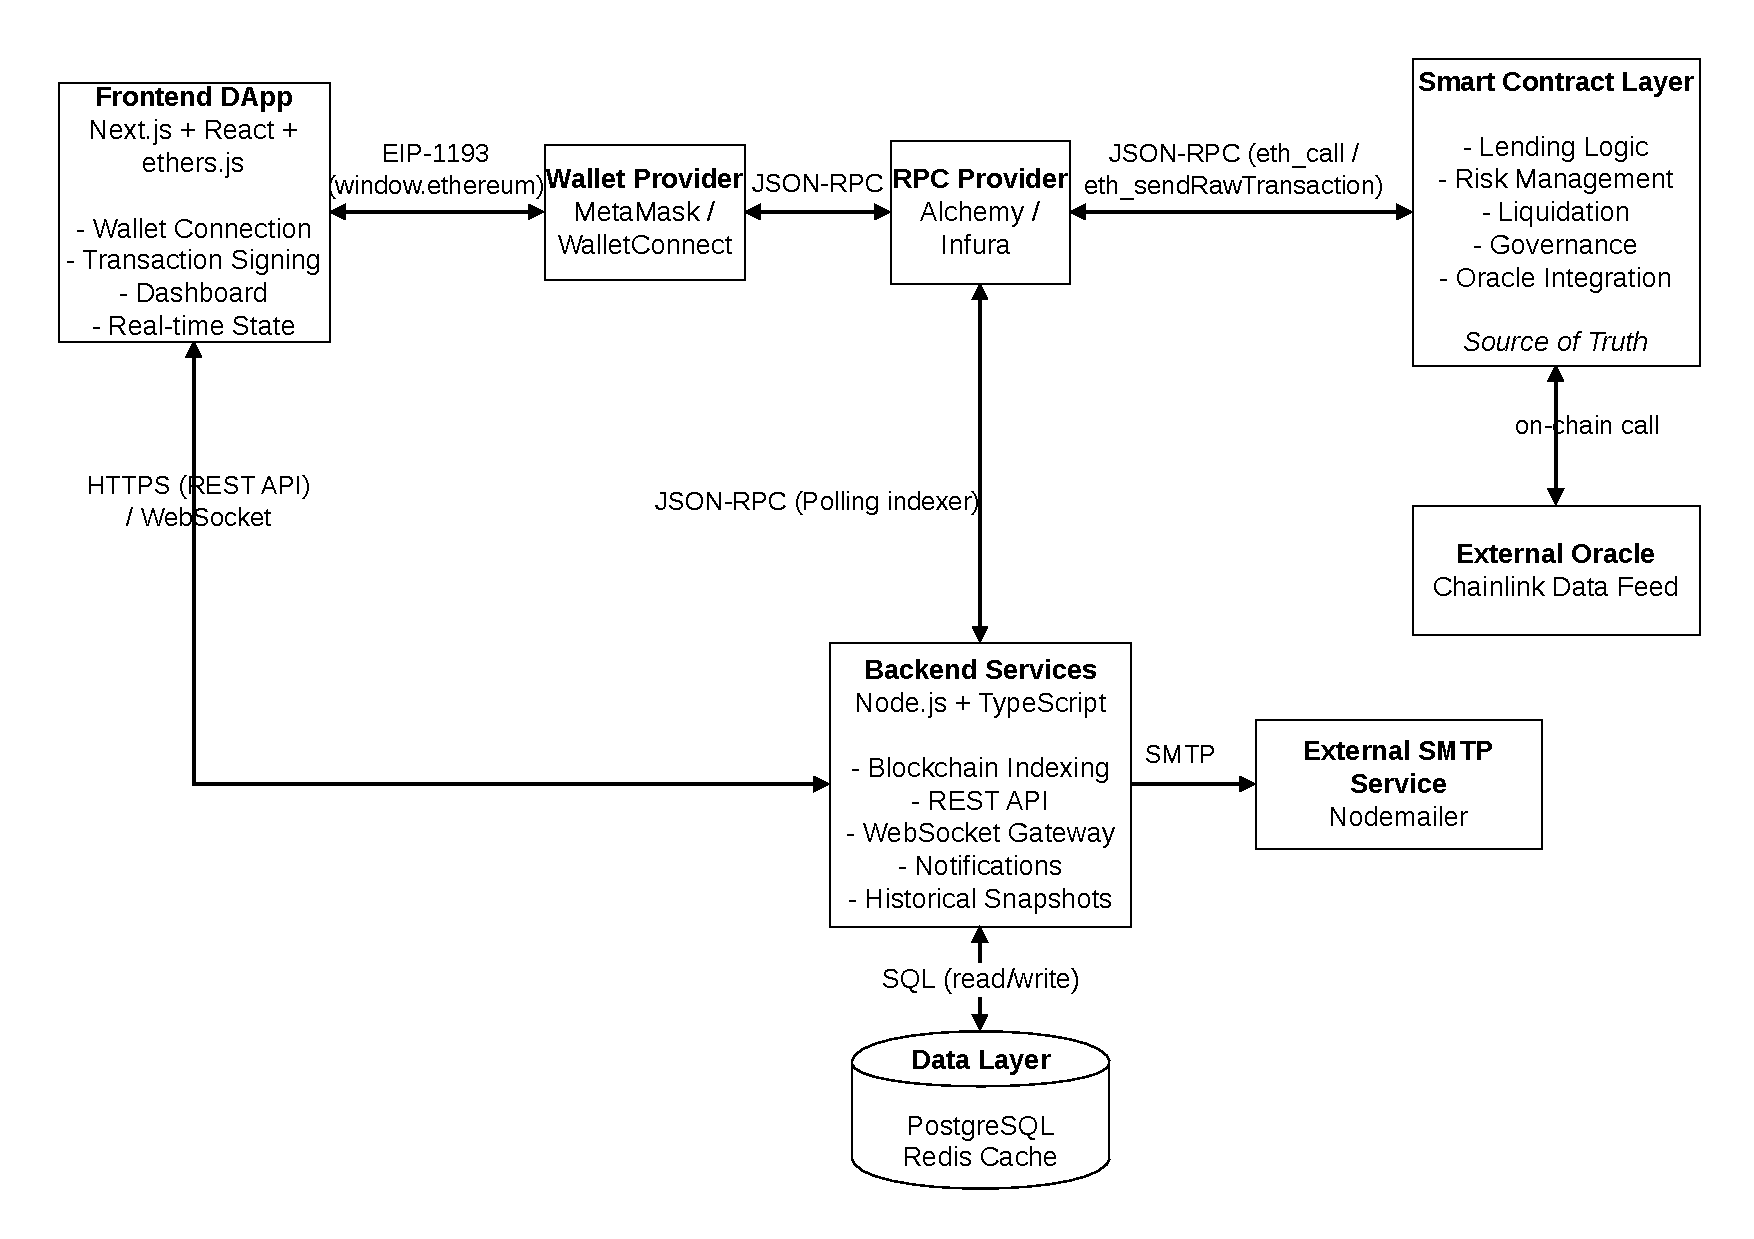
\includegraphics[
    page=1,
    width=\textwidth,
    height=0.9\textheight,
    keepaspectratio
]{../Hinhve/STACTT.pdf}
\caption{Sơ đồ kiến trúc tổng quan hệ thống}
\label{fig:system_architecture}
\end{figure}


\section{Thiết kế hợp đồng thông minh (Smart contract)}


Giao thức mà đồ án này xây dựng gồm có tổng cộng 5 smart contract logic chính. Thông thường, khi đã triển khai một smart contract on-chain, smart contract đó là bất biến, các hàm logic không thể thay đổi, tuy nhiên, trong giao thức của đồ án, có 2 smart contract được thiết kế theo hướng có thể cập nhật mới logic, kỹ thuật được lựa chọn sử dụng ở đây chính là UUPS (Universal Upgradeable Proxy Standard)~\cite{EIP1822,OpenZeppelinDocs}, chia một contract thành hai phần: một implementation contract (logic) và một proxy contract (storage). Sau đây là sơ bộ tổng quan về các smart contract được triển khai: (i) LendingPool / LendingPoolStorage: smart contract quan trọng nhất của giao thức, đảm nhiệm đa số các chức năng chính (gửi/ vay/ rút/ trả tài sản), thực hiện lazy accrual (tích lũy lãi suất chỉ khi người dùng tương tác); chứa logic cho phép admin quản lý tài sản và ngân quỹ; cung cấp các hàm tiện ích để phục vụ cho UI, UX, đồng thời lưu trữ toàn bộ các thông tin về các số dư tài sản, người dùng trong giao thức. (ii) Liquidation: đảm nhận chức năng thanh lý vị thế của giao thức, chịu trách nhiệm cho các tham số rủi ro, các hàm phục vụ cho việc phát hiện vị thế rơi vào ngưỡng thanh lý và thực hiện quá trình thanh lý. (iii) InterestRateModel: đảm nhận xử lý mô hình lãi suất của giao thức, tính lãi gửi, lãi vay của từng tài sản được hỗ trợ trong giao thức, smart contract này là một smart contract độc lập, không phụ thuộc vào các smart contract khác trong hệ thống, chỉ có chức năng tính và cung cấp lãi suất vay và gửi tương ứng. (iv) PriceRouter/ PriceRouterStorage: hoạt động giống như một bộ định tuyến quyết định xem sử dụng giá từ MyOracle hay từ Oracle thật (Chainlink), từ đó cung cấp giá cho các loại tài sản khác nhau trong giao thức~\cite{ChainlinkDocs}. (v) MyOracle: để tự cung cấp giá cho các tài sản trong giao thức.

Bên cạnh các smart contract phục vụ cho nghiệp vụ logic, giao thức còn có thêm 2 smart contract nhằm mục đích quản trị giao thức, đó là ProtocolController, làm entrypoint cho admin để thực thi quyền quản trị và cài đặt đối với các smart contract khác trong giao thức và TimelockController, dùng để áp đặt timelock (khóa thời gian) cho các động thái của admin tác động đến giao thức nhằm đảm bảo tính minh bạch cho giao thức. Ngoài ra còn có 1 smart contract nữa là MockERC20 - token giả định để có thể kiểm thử. Khi đã xác định xong bộ khung của giao thức, tiến hành xây dựng từng smart contract một, bao gồm các biến (state), các cấu trúc dữ liệu, các hàm logic nghiệp vụ chính, xác định một smart contract sẽ cần phải tương tác với các smart contract nào (ở đây, đồ án lựa chọn hướng thiết kế đó là thay vì chỉ lưu địa chỉ smart contract ở ProtocolController thì lưu cả địa chỉ các smart contract ở nội bộ smart contract, tuy đánh đổi bởi việc phải lưu ở nhiều chỗ hơn, khi cập nhật địa chỉ smart contract mới thì cần phải ghi nhiều hơn, nhưng khi đọc thì các smart contract có thể tự lấy địa chỉ nhanh chóng mà không cần một RPC call sang ProtocolController).

Trước khi đi vào chi tiết từng smart contract, cần nắm được bức tranh tổng thể về cách các smart contract tương tác với nhau trong giao thức (được biểu diễn bằng hình~\ref{fig:smart_contract_architecture}). Mỗi smart contract đảm nhận một vai trò rõ ràng và chỉ giao tiếp với các smart contract khác thông qua các interface đã được định nghĩa trước.

ProtocolController là điểm vào duy nhất (single entry point) cho mọi hành động quản trị. Tất cả các lệnh cấu hình, cập nhật tham số hay nâng cấp đều phải đi qua smart contract này trước khi được chuyển tiếp đến các smart contract khác như LendingPool, Liquidation, PriceRouter và MyOracle.

LendingPool là trung tâm của giao thức, lưu trữ toàn bộ trạng thái tài sản và vị thế người dùng. Contract này chỉ chấp nhận lệnh từ hai nguồn: ProtocolController (các hàm admin) và Liquidation (hai hook thanh lý seizeCollateral và repayFromLiquidation). Khi cần tính toán liên quan đến giá hoặc lãi suất, LendingPool gọi ra ngoài đến PriceRouter và InterestRateModel tương ứng.

Liquidation đọc trạng thái vị thế người dùng từ LendingPool, lấy giá từ PriceRouter, rồi gọi ngược lại hai hook của LendingPool để cập nhật số dư trong quá trình thanh lý. Contract này không tự lưu trữ bất kỳ số dư nào của người dùng.

PriceRouter là lớp trừu tượng hóa nguồn giá (Oracle Abstraction Layer), được gọi bởi cả LendingPool và Liquidation. Không smart contract nào gọi trực tiếp Chainlink hay MyOracle --- mọi truy vấn giá đều đi qua PriceRouter.getPrice().

InterestRateModel là contract thuần tính toán (stateless), chỉ được gọi bởi LendingPool khi cần lấy lãi suất vay và gửi. Không phụ thuộc vào bất kỳ smart contract nào khác trong hệ thống.

\begin{figure}[H]
\centering
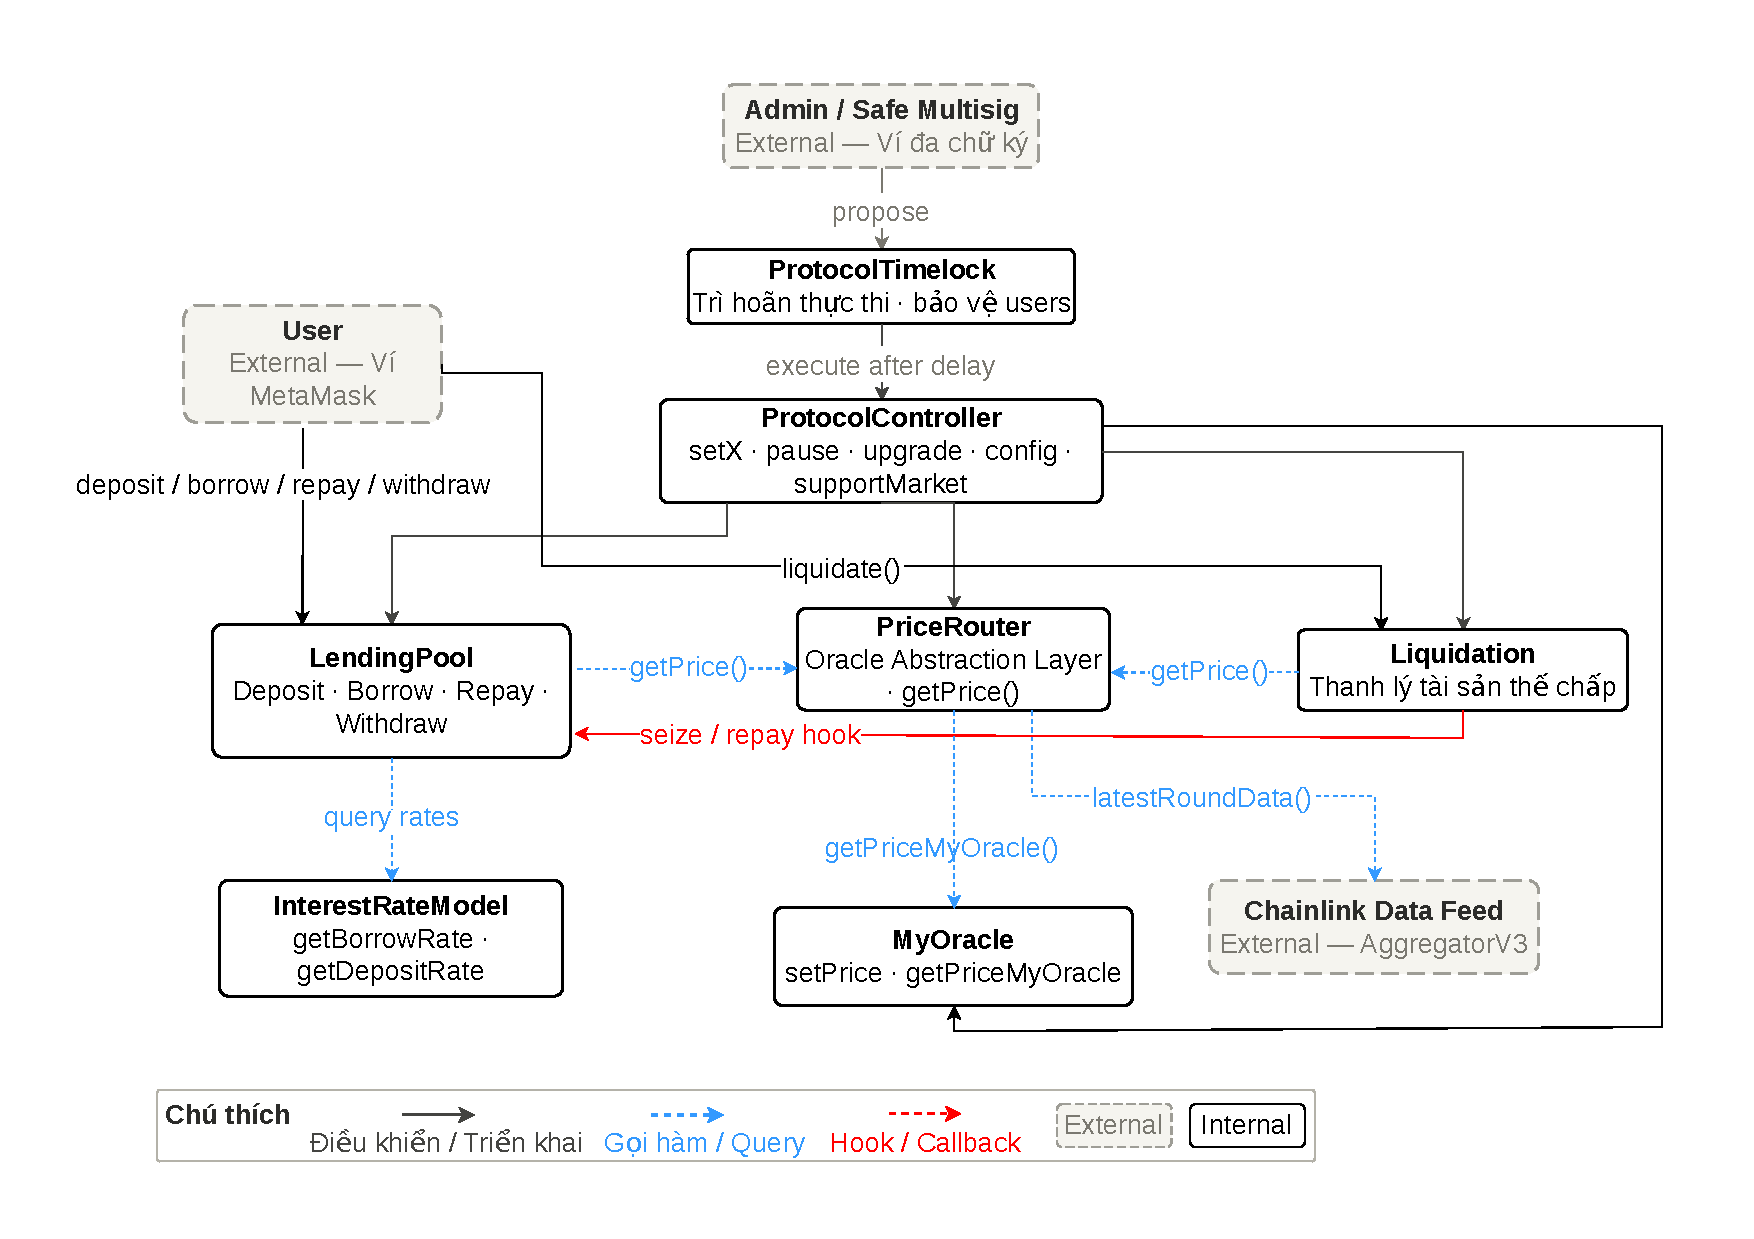
\includegraphics[
    page=1,
    width=\textwidth,
    height=0.9\textheight,
    keepaspectratio
]{../Hinhve/SCACTT.pdf}
\caption{Tổng quan kiến trúc smart contract}
\label{fig:smart_contract_architecture}
\end{figure}


\subsection{LendingPool / LendingPoolStorage}


\subsubsection{Mô hình dữ liệu (Data Model)}


LendingPool là smart contract nền tảng của toàn bộ giao thức, lưu trữ tài sản của giao thức và vị thế của người dùng, smart contract này được thiết kế với hai struct chính, đầu tiên chính là Struct Market, được trình bày trong bảng~\ref{table:market_struct}, đây là trạng thái của một tài sản trong giao thức:

\begin{table}[H]
\centering
\resizebox{\textwidth}{!}{%
\begin{tabular}{|p{0.27\textwidth}|p{0.73\textwidth}|}
\hline
\textbf{Trường} & \textbf{Ý nghĩa} \\ \hline
isSupported & Tài sản có đang được kích hoạt không \\ \hline
totalDeposits & Tổng gốc + lãi tích lũy đã gửi (tăng theo thời gian) \\ \hline
totalBorrows & Tổng gốc + lãi tích lũy đang vay (tăng theo thời gian) \\ \hline
borrowIndex & Chỉ số tích lũy lãi vay (bắt đầu = 1e18) \\ \hline
depositIndex & Chỉ số tích lũy lãi gửi (bắt đầu = 1e18) \\ \hline
lastUpdateTimestamp & Thời điểm cập nhật lãi suất cuối cùng \\ \hline
interestRateModel & Địa chỉ smart contract tính lãi suất \\ \hline
\end{tabular}
}
\caption{Struct Market của LendingPool}
\label{table:market_struct}
\end{table}


Tiếp theo là Struct Balance, được trình bày ở bảng~\ref{table:balance_struct}, là vị thế của một người dùng đối với 1 tài sản

\begin{table}[H]
\centering
\resizebox{\textwidth}{!}{%
\begin{tabular}{|p{0.28\textwidth}|p{0.72\textwidth}|}
\hline
\textbf{Trường} & \textbf{Ý nghĩa} \\ \hline
deposited & Số dư gốc tại thời điểm snapshot \\ \hline
borrowed & Số nợ gốc tại thời điểm snapshot \\ \hline
borrowIndexSnapShot & Giá trị borrowIndex tại lần tương tác cuối \\ \hline
depositIndexSnapShot & Giá trị depositIndex tại lần tương tác cuối \\ \hline
\end{tabular}
}
\caption{Struct Balance của LendingPool}
\label{table:balance_struct}
\end{table}


Trạng thái của giao thức được lưu trữ thông qua các map và array, tiêu biểu có thể kể đến như các cấu trúc dữ liệu trong bảng~\ref{table:data_structures}.

\begin{table}[H]
\centering
\resizebox{\textwidth}{!}{%
\begin{tabular}{|p{0.22\textwidth}|p{0.38\textwidth}|p{0.40\textwidth}|}
\hline
\textbf{State} & \textbf{Cấu trúc dữ liệu} & \textbf{Ý nghĩa} \\ \hline
markets & mapping(address => Market) & Theo dõi trạng thái của từng tài sản (asset => Market) \\ \hline
userBalances & mapping(address => mapping(address => Balance)) & Theo dõi trạng thái của từng người dùng với từng tài sản (user => asset => Balance) \\ \hline
userMarkets & mapping(address => address[]) & Lưu trữ địa chỉ toàn bộ tài sản mà người dùng tương tác (user => list of assets) \\ \hline
treasuryBalances & mapping(address => uint256) & Lưu trữ ngân quỹ của từng tài sản (asset => amount) \\ \hline
userMarketExists & mapping(address => mapping(address => bool)) & Mapping để tránh push duplicate vào userMarkets array \\ \hline
\end{tabular}
}
\caption{Cấu trúc dữ liệu tiêu biểu}
\label{table:data_structures}
\end{table}


Quan trọng, LendingPoolStorage khai báo \mbox{\texttt{\_\_gap[39]}} để dự trữ slot cho UUPS upgrade --- đây là best practice bắt buộc khi dùng upgradeable pattern. Lý thuyết về rủi ro xung đột slot đã trình bày tại mục~\ref{section:3.4.4}; chi tiết phân bổ slot cụ thể tại mục~\ref{section:6.1.3.b}.

\subsubsection{Cơ chế tích lũy lãi suất}
\label{section:4.2.1.b}


Cơ chế tích lũy lãi suất theo thời gian là điểm nổi bật và quan trọng nhất của giao thức, là trái tim của contract. Hai tính chất --- không kỳ hạn và lãi suất thả nổi --- tạo ra bài toán tích lũy lãi liên tục: tại mỗi thời điểm, số dư thực tế của người dùng bằng số tiền gốc cộng với toàn bộ lãi đã tích lũy từ lần tương tác cuối đến hiện tại, với lãi suất có thể đã thay đổi nhiều lần trong khoảng đó. Giao thức giải quyết bài toán này thông qua cơ chế Lazy Accrual (tích lũy lãi trễ) cùng với Global Interest Index (chỉ số lãi toàn cục). Cơ chế này hoạt động dựa vào 2 struct Market (borrowIndex, depositIndex) và struct Balance (borrowIndexSnapShot, depositIndexSnapShot), Lazy Accrual đảm bảo chỉ khi có người dùng tương tác với một loại tài sản, hàm accrueInterest(address asset) mới được thực thi và tiến hành tích lũy lãi suất cho tài sản đó. Cách thực hoạt động: accrueInterest sẽ tiến hành thu thập lãi suất và tiến hành tích lũy cho số dư thực tế và chỉ số index cho một loại tài sản, bao gồm cả phía vay và phía gửi, đồng thời phần dư ra sẽ được đưa vào ngân quỹ của tài sản:
\begin{align}
\mathrm{interestAccrued} &= \mathrm{totalBorrows} \times r_{\mathrm{borrow}} \times \frac{\Delta t}{\mathrm{SECONDS\_PER\_YEAR} \times S} \label{eq:interest_accrued} \\
\mathrm{borrowIndex} &\mathrel{+}= \mathrm{borrowIndex} \times r_{\mathrm{borrow}} \times \frac{\Delta t}{\mathrm{SECONDS\_PER\_YEAR} \times S} \label{eq:borrow_index} \\
\mathrm{depositInterest} &= \mathrm{totalDeposits} \times r_{\mathrm{deposit}} \times \frac{\Delta t}{\mathrm{SECONDS\_PER\_YEAR} \times S} \label{eq:deposit_interest} \\
\mathrm{depositIndex} &\mathrel{+}= \mathrm{depositIndex} \times r_{\mathrm{deposit}} \times \frac{\Delta t}{\mathrm{SECONDS\_PER\_YEAR} \times S} \label{eq:deposit_index} \\
\mathrm{toTreasury} &= \mathrm{interestAccrued} - \mathrm{depositInterest} \label{eq:to_treasury}
\end{align}

Trong đó, $S = 10^{18}$ là hằng số SCALE, $\Delta t$ là số giây đã trôi qua kể từ lần cập nhật cuối, và $\mathrm{toTreasury}$ là phần spread giữ lại cho ngân quỹ giao thức.


Đối với vị thế của người dùng được lưu trong Balance, giao thức sẽ tiến hành tích lũy một phía (nghĩa là nếu người dùng gửi thêm hoặc rút thì tích lũy Deposit, nếu vay hoặc trả nợ thì tích lũy Borrow):

\begin{align}
\mathrm{currentUserDeposit} &= \mathrm{deposited} \times \frac{\mathrm{depositIndex}}{\mathrm{depositIndexSnapShot}} \label{eq:current_deposit} \\
\mathrm{currentUserBorrow} &= \mathrm{borrowed} \times \frac{\mathrm{borrowIndex}}{\mathrm{borrowIndexSnapShot}} \label{eq:current_borrow}
\end{align}


Lý do lựa chọn Lazy Accrual thay vì Eager Accrual, cùng với phân tích so sánh Global Interest Index với các cách tiếp cận thay thế, được trình bày chi tiết tại mục~\ref{section:5.1}. Kỹ thuật số học fixed-point phục vụ cài đặt các công thức trên được trình bày tại mục~\ref{section:6.1.3.a}.

\subsubsection{Các chức năng nghiệp vụ chính (Core Functions)}


Giao thức có tổng cộng là 4 hàm nghiệp vụ chính, tương đương với 4 chức năng chính của giao thức, được liệt trong bảng~\ref{table:core_functions}, luồng hoạt động của các chức được thể hiện lần lượt ở các hình~\ref{fig:df}, \ref{fig:bf}, \ref{fig:rf} và \ref{fig:wf}.

\begin{table}[H]
\centering
\resizebox{\textwidth}{!}{%
\begin{tabular}{|p{0.49\textwidth}|p{0.51\textwidth}|}
\hline
\textbf{Hàm} & \textbf{Chức năng} \\ \hline
deposit(address asset, uint amount) & Gửi tài sản vào giao thức để nhận lãi \\ \hline
borrow(address asset, uint amount) & Vay tài sản dựa trên tài sản thế chấp \\ \hline
repay(address asset, uint amount) & Trả nợ vay \\ \hline
withdraw(address asset, uint amount) & Rút tài sản đã gửi \\ \hline
\end{tabular}
}
\caption{Các hàm nghiệp vụ chính}
\label{table:core_functions}
\end{table}


\begin{figure}[H]
\centering
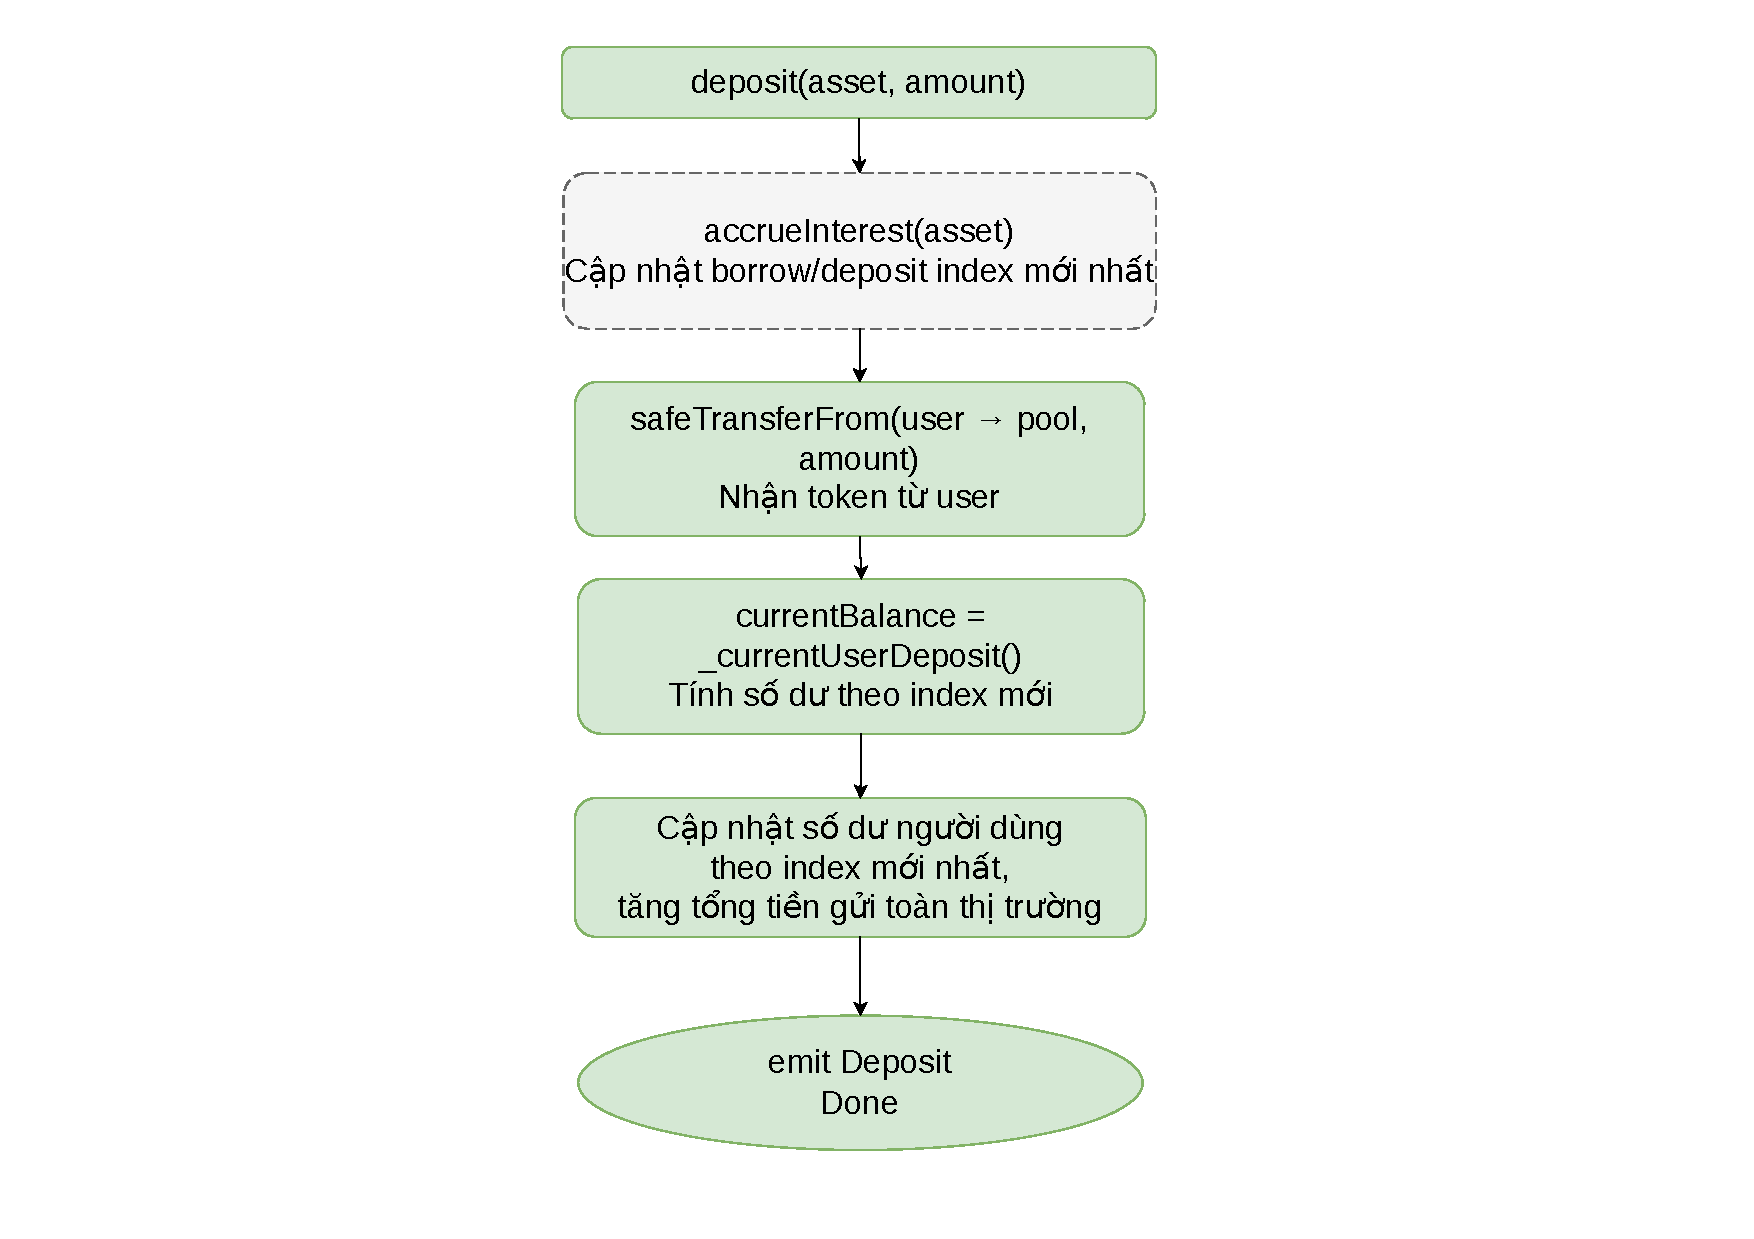
\includegraphics[
    page=1,
    width=\textwidth,
    height=0.9\textheight,
    keepaspectratio
]{../Hinhve/DF.pdf}
\caption{Sơ đồ luồng gửi tài sản}
\label{fig:df}
\end{figure}


\begin{figure}[H]
\centering
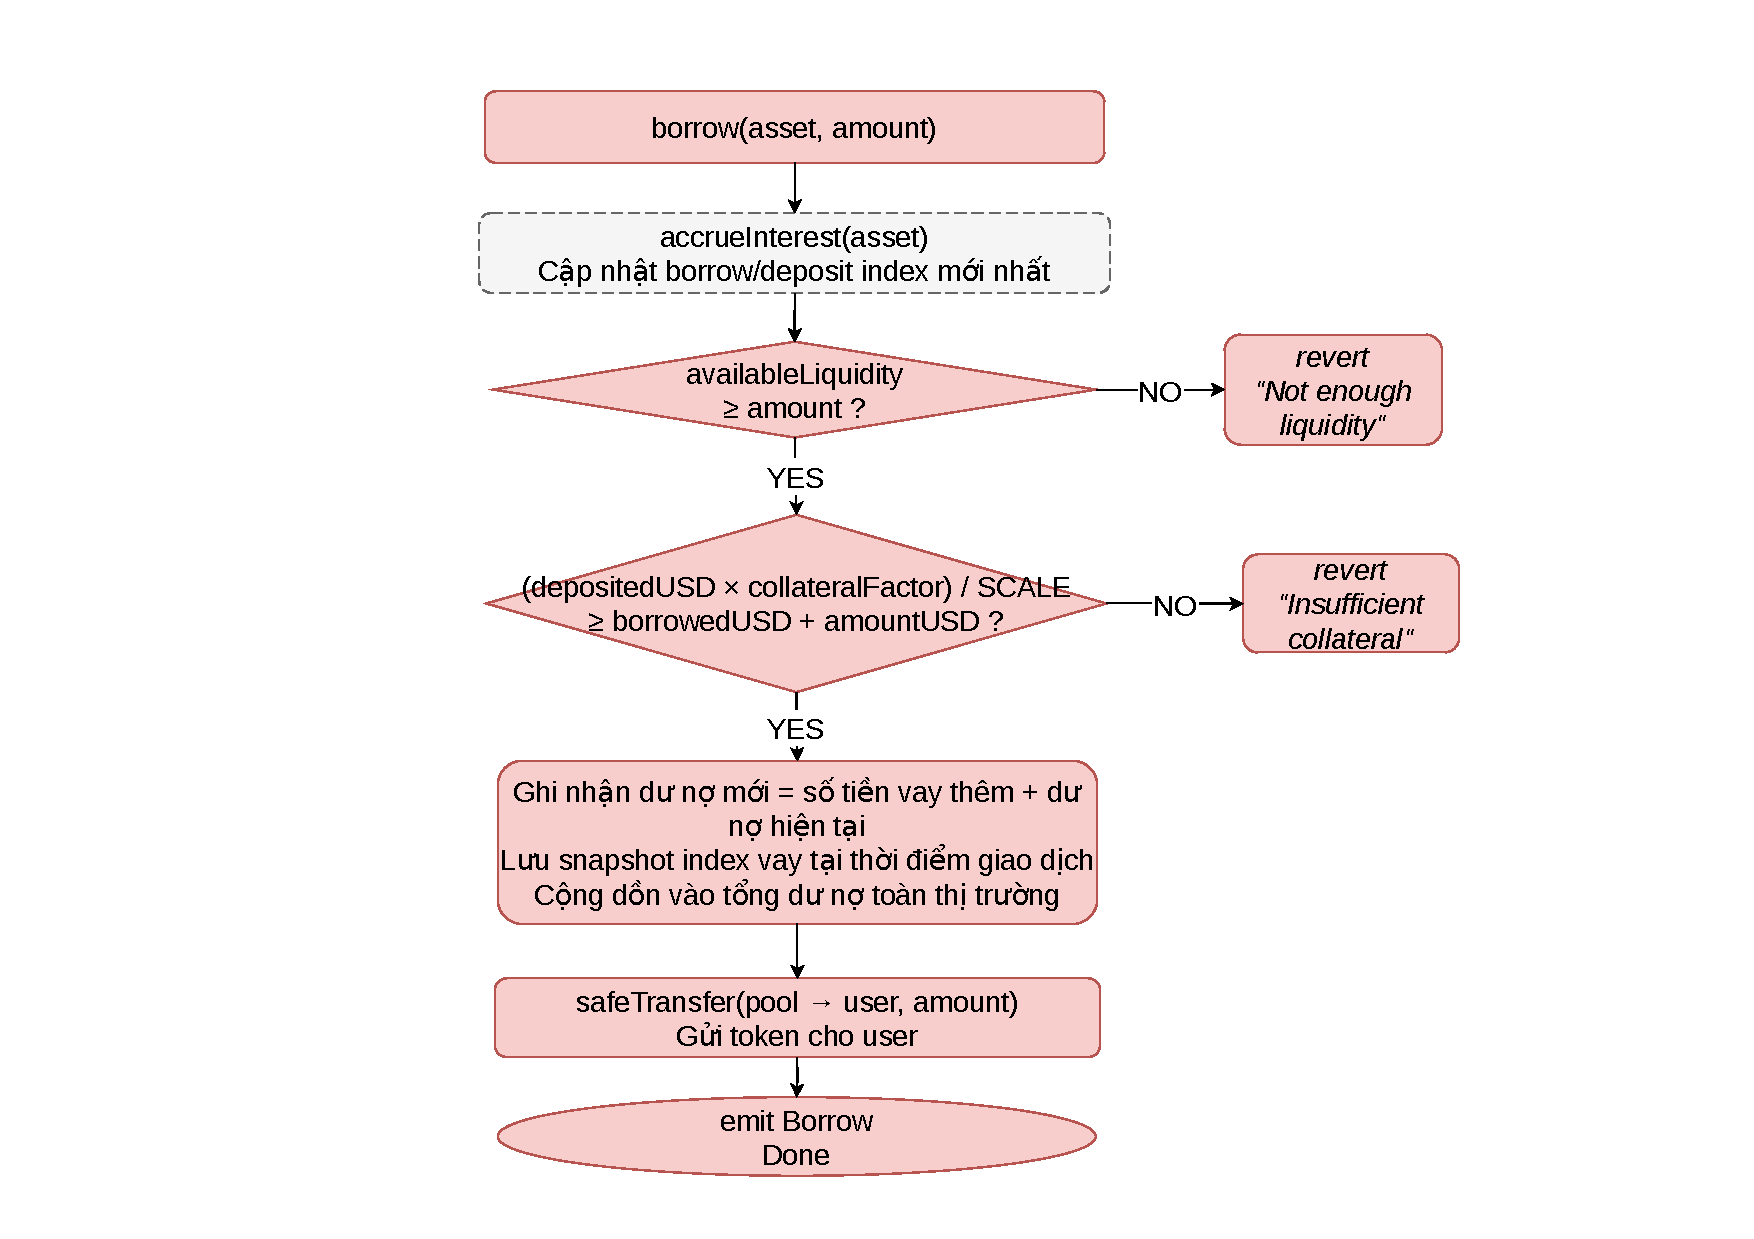
\includegraphics[
    page=1,
    width=\textwidth,
    height=0.9\textheight,
    keepaspectratio
]{../Hinhve/BF.pdf}
\caption{Sơ đồ luồng vay tài sản}
\label{fig:bf}
\end{figure}


\begin{figure}[H]
\centering
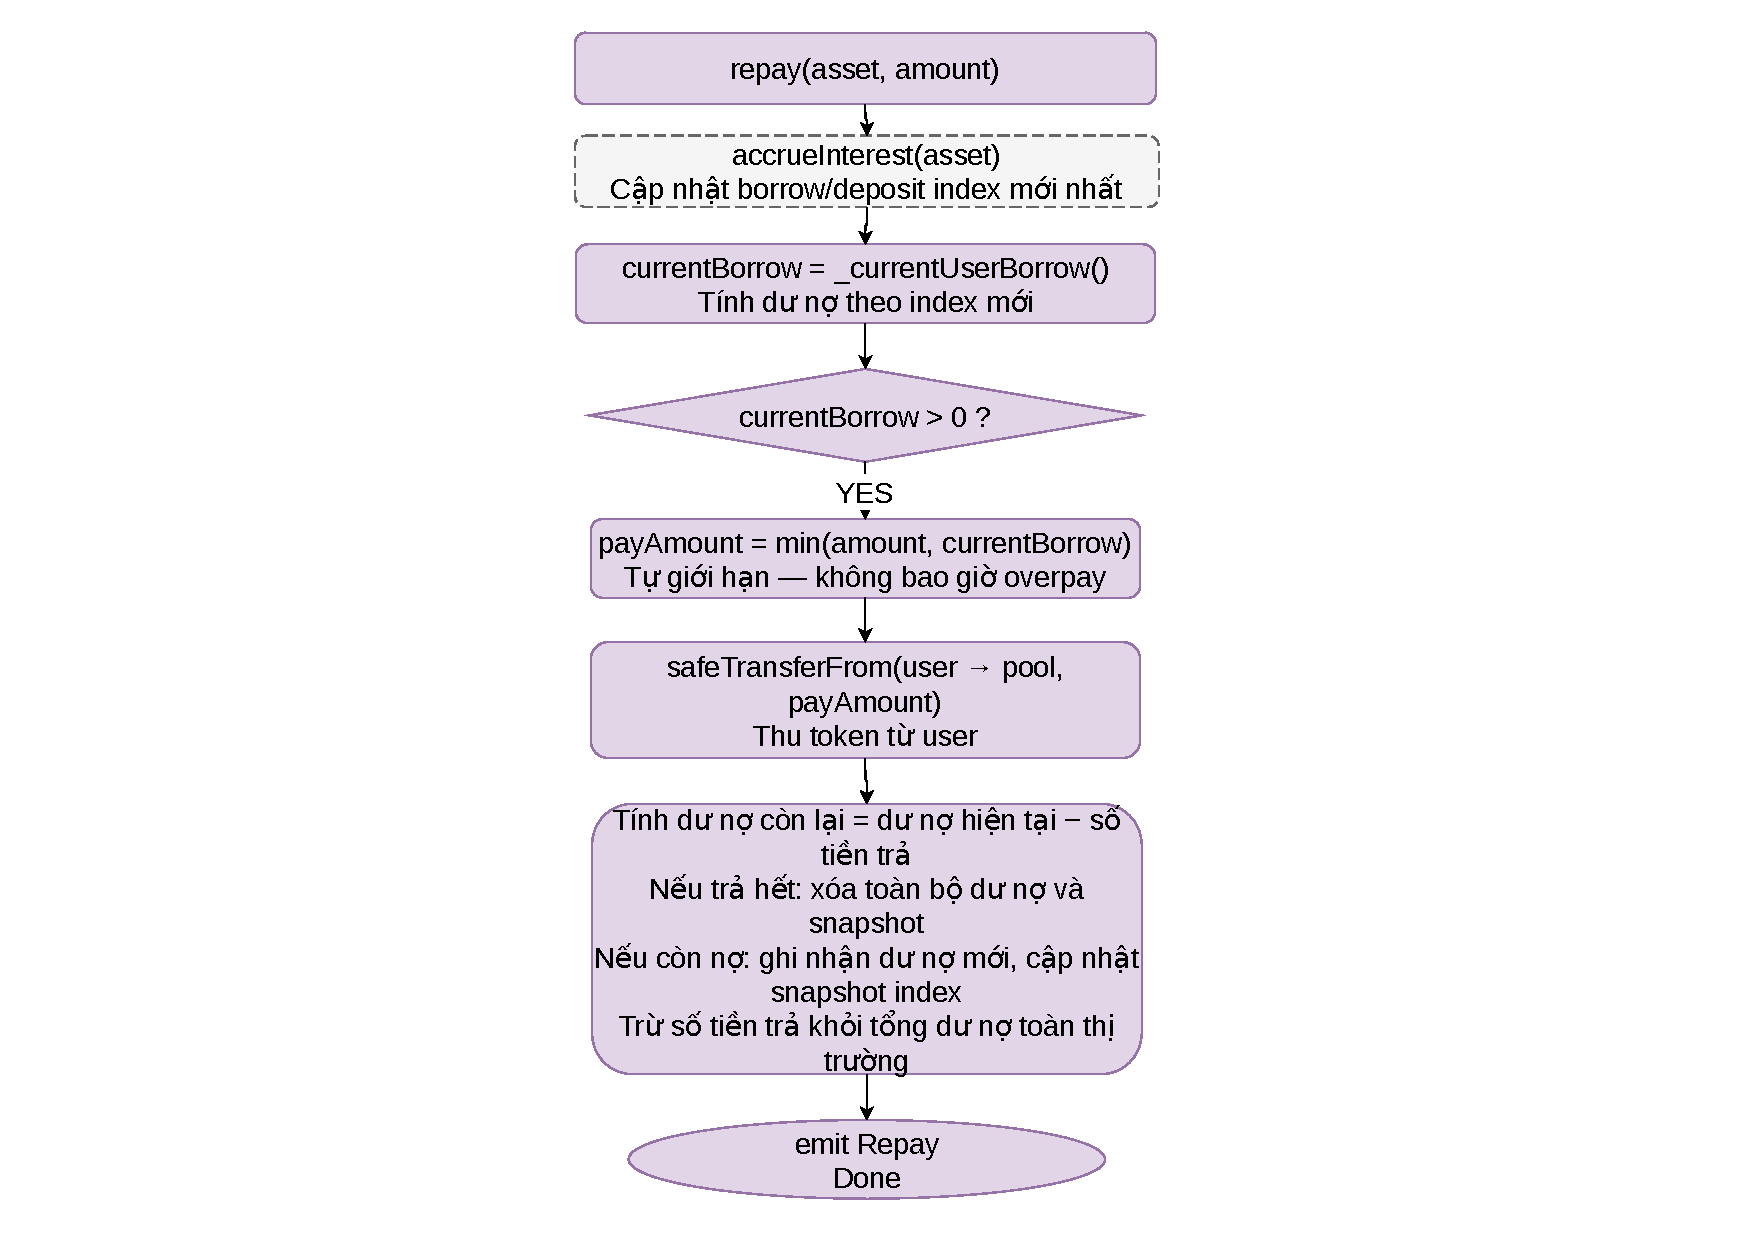
\includegraphics[
    page=1,
    width=\textwidth,
    height=0.9\textheight,
    keepaspectratio
]{../Hinhve/RF.pdf}
\caption{Sơ đồ luồng trả nợ}
\label{fig:rf}
\end{figure}


\begin{figure}[H]
\centering
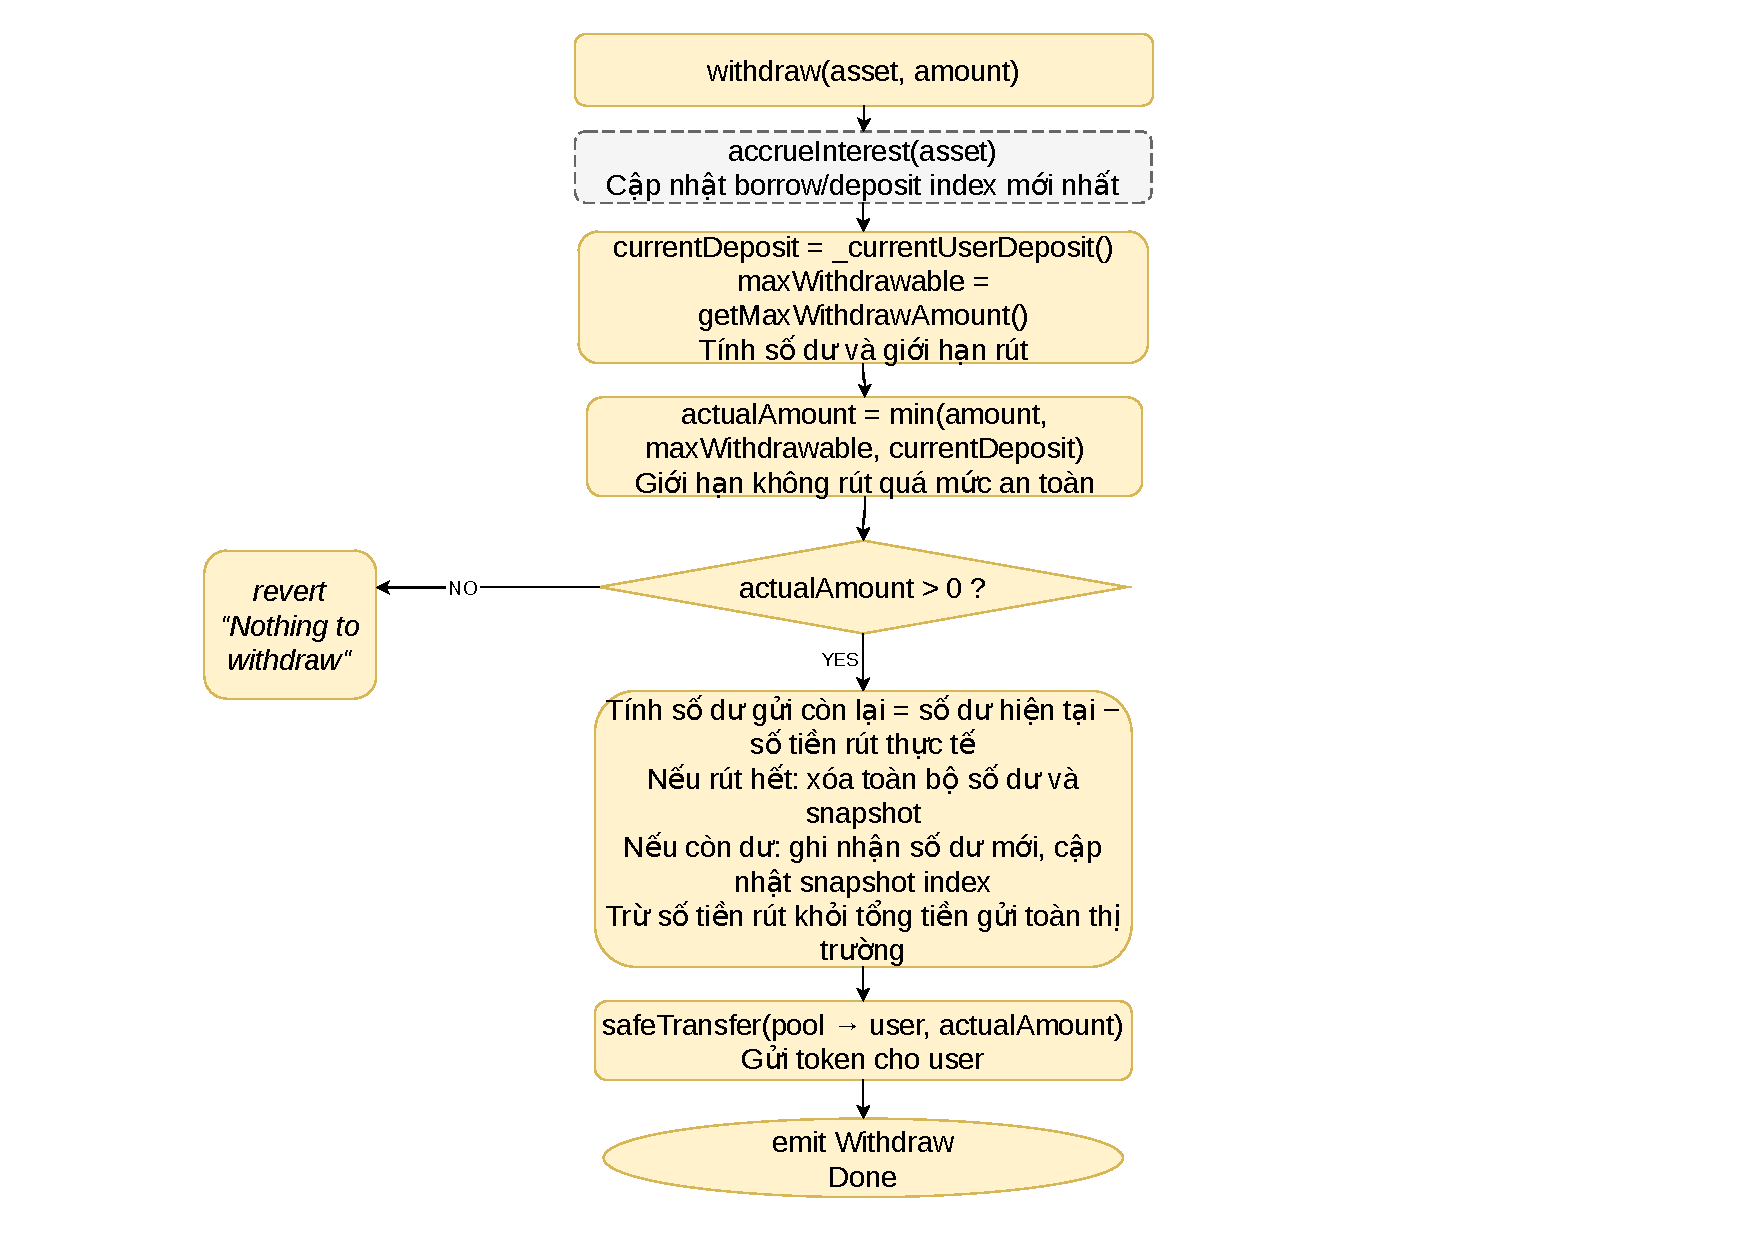
\includegraphics[
    page=1,
    width=\textwidth,
    height=0.9\textheight,
    keepaspectratio
]{../Hinhve/WF.pdf}
\caption{Sơ đồ luồng rút tài sản}
\label{fig:wf}
\end{figure}


\subsubsection{Cơ chế bảo mật (Security Mechanism)}
\label{section:4.2.1.a}


Bề mặt tấn công của một lending protocol bao gồm nhiều lớp rủi ro khác nhau: reentrancy attack ở tầng EVM, chiếm quyền khởi tạo proxy, truy cập trái phép hàm admin, lỗi logic nghiệp vụ, và rút cạn thanh khoản treasury. Mỗi loại rủi ro này đòi hỏi một cơ chế phòng vệ riêng biệt --- không có cơ chế nào bảo vệ được toàn bộ. Do đó, LendingPool được thiết kế bảo mật theo 5 tầng độc lập, mỗi tầng phòng vệ một lớp rủi ro cụ thể.

Tầng 1: Bảo vệ cấp contract (Contract-level), dùng các thư viện đã được audit, kiểm chứng của Openzeppelin, đầu tiên là chống lại tấn công reentrancy sử dụng ReentrancyGuardTransient, áp dụng nonReentrant cho toàn bộ các hàm state-changing (deposit, borrow, repay, withdraw, seizeCollateral, repayFromLiquidation); SafeERC20 cho tất cả lệnh transfer token đều qua safeTransferFrom / safeTransfer thay vì gọi trực tiếp transfer. Điều này xử lý các ERC20 không chuẩn: một số token không trả về bool hoặc trả về false thay vì revert khi thất bại, SafeERC20 sẽ wrap lại và revert nếu token báo lỗi; PausableUpgradeable hết hợp whenNotPaused: tất cả hàm user-facing và accrueInterest đều có guard whenNotPaused; khi admin kích hoạt pause, toàn bộ giao thức đóng băng ngay lập tức, không thể deposit, borrow, repay, withdraw, hay tích lũy lãi.

Tầng 2: Bảo vệ khởi tạo (Initialization Safety), \_disableInitializers() trong constructor làm cho implementation contract (không phải proxy) bị khóa cứng, không thể gọi initialize(). Nếu không có dòng này, kẻ tấn công có thể khởi tạo implementation trực tiếp và chiếm quyền controller. Modifier initializer sẽ đảm bảo initialize() chỉ được gọi đúng một lần trên proxy, các lần gọi tiếp theo đều bị revert.

Tầng 3: Phân quyền truy cập (Access Control), tầng này sử dụng các modifier để định nghĩa quyền truy cập và ngăn chặn các truy cập trái phép, các modifier được thể hiện trong bảng~\ref{table:access_control_modifiers}.

\begin{table}[H]
\centering
\resizebox{\textwidth}{!}{%
\begin{tabular}{|p{0.34\textwidth}|p{0.32\textwidth}|p{0.33\textwidth}|}
\hline
\textbf{Modifier} & \textbf{Áp dụng cho} & \textbf{Ý nghĩa bảo vệ} \\ \hline
onlyController & Toàn bộ hàm admin & Chỉ ProtocolController (và sau đó là Timelock) mới được thay đổi cấu hình \\ \hline
onlyLiquidation & seizeCollateral, repayFromLiquidation & Chỉ Liquidation contract mới được gọi hook --- không ai có thể tùy ý xóa collateral của người khác \\ \hline
\_authorizeUpgrade override với onlyController & UUPS upgrade & Chỉ controller mới được nâng cấp implementation, không ai khác \\ \hline
\end{tabular}
}
\caption{Các modifier phân quyền truy cập}
\label{table:access_control_modifiers}
\end{table}


Lưu ý thiết kế: hai hook thanh lý được bảo vệ bởi onlyLiquidation chứ không phải onlyController, vì trong runtime, controller không phải người gọi các hàm này, Liquidation contract mới là người gọi trực tiếp.

Tầng 4: Kiểm soát nghiệp vụ (Business Logic Guards), được cài đặt trực tiếp bên trong các hàm tương tác với giao thức, sử dụng để đảm bảo nghiệp vụ của giao thức được thực hiện một cách chính xác mà không có lỗi gì có thể khai thác

Trong \texttt{borrow()}:
\begin{itemize}
  \item Kiểm tra thanh khoản thị trường: amount $\leq$ totalDeposits + treasury - totalBorrows --- không được vay quá số token thực có trong pool.
  \item Kiểm tra đủ tài sản thế chấp: totalDepositedUSD $\times$ collateralFactor / SCALE $\geq$ totalBorrowedUSD + amountUSD --- collateral phải đủ cover khoản vay mới.
\end{itemize}

Trong \texttt{repay()}:
\begin{itemize}
  \item Auto-cap số tiền trả: Nếu amount $>$ currentBorrow thì payAmount = currentBorrow --- người dùng không bao giờ trả nhiều hơn số nợ thực tế, tránh mất tiền do nhập nhầm số.
\end{itemize}

Trong \texttt{withdraw()}:
\begin{itemize}
  \item Giới hạn rút bởi collateral: actualAmount = min(amount, getMaxWithdrawAmount()) --- không cho phép rút phần collateral đang cover nợ, đảm bảo vị thế luôn trên ngưỡng an toàn.
  \item Giới hạn rút bởi số dư thực: actualAmount = min(actualAmount, currentDeposit) --- không rút quá số dư hiện có.
\end{itemize}

Trong \texttt{seizeCollateral()} (liquidation hook):
\begin{itemize}
  \item currentBorrowerDeposit $\geq$ seizeAmount --- không thể seize nhiều hơn số collateral borrower đang có.
\end{itemize}

Trong \texttt{repayFromLiquidation()} (liquidation hook):
\begin{itemize}
  \item repayAmount $\leq$ currentBorrow --- không thể repay nhiều hơn số nợ thực (Liquidation contract đã cap trước với maxRepayAmount (currentBorrow \* closeFactor), nhưng LendingPool vẫn kiểm tra độc lập --- defense in depth).
\end{itemize}

Trong \texttt{accrueInterest()}:
\begin{itemize}
  \item Guard timeElapsed == 0 --- nếu đã tích lũy lãi trong cùng block thì return sớm, tránh tích lũy hai lần.
\end{itemize}


Tầng 5: Bảo vệ ngân quỹ giao thức (Protocol Treasury Safety)

withdrawTreasury() --- trước khi rút tiền từ treasury, kiểm tra bất biến:
\begin{equation}
\mathrm{totalDeposits} + \mathrm{treasuryBalances} - \mathrm{amount} \geq \mathrm{totalBorrows}
\label{eq:treasury_invariant}
\end{equation}


Nghĩa là dù treasury bị rút, tổng tài sản trong pool vẫn phải đủ cover toàn bộ nợ đang được vay. Admin không thể rút cạn thanh khoản và để lại người gửi không rút được.

rescueToken() --- chỉ cho phép rút phần surplus --- token dư ra không được hạch toán trong bất kỳ vị thế nào:
\begin{equation}
\mathrm{surplus} = \mathrm{balanceOf(contract)} - (\mathrm{totalDeposits} + \mathrm{treasuryBalances})
\label{eq:rescue_surplus}
\end{equation}


Token của người dùng và treasury không bao giờ bị động đến. Hàm này xử lý trường hợp ai đó gửi nhầm token vào địa chỉ contract.

Ngoài các hàm quản lý ngân quỹ dành riêng cho admin, LendingPool còn cung cấp hàm donate(asset, amount) cho phép bất kỳ ai đóng góp token vào treasuryBalances của một tài sản đang được hỗ trợ, mà không làm thay đổi totalDeposits hay totalBorrows, từ đó không pha loãng utilization rate của giao thức, tránh tác động đến lãi suất của giao thức. Ứng dụng thực tế của hàm này bao gồm: nhóm phát triển bơm thêm thanh khoản dự phòng trong giai đoạn đầu khi lượng người dùng còn ít, hoặc cộng đồng bổ sung nguồn lãi để kích thích người gửi tài sản. Mặc dù mở với tất cả mọi người, hàm donate vẫn được bảo vệ bởi nonReentrant, whenNotPaused và onlySupportedMarket, đảm bảo không thể donate vào asset không hợp lệ hoặc khi giao thức đang tạm dừng khẩn cấp.

Phân tích lý do chọn thiết kế phân tầng thay vì validate tập trung, cùng với các quyết định thiết kế phi hiển nhiên trong cơ chế bảo mật, được trình bày tại mục~\ref{section:5.2}.

\subsubsection{Liquidation Hooks \& Mô hình phân tách trách nhiệm}


Hai hàm seizeCollateral() và repayFromLiquidation() chỉ được gọi bởi Liquidation contract (onlyLiquidation). Đây là thiết kế separation of concerns:

\begin{itemize}
  \item LendingPool quản lý balance/state.
  \item Liquidation chứa toàn bộ logic thanh lý.
  \item LendingPool chỉ expose hook để Liquidation gọi vào cập nhật state.
\end{itemize}


\subsubsection{View/Preview Functions --- phục vụ UX}


Nhóm hàm này không thay đổi state, dùng để frontend hiển thị real-time, thể hiện dưới bảng~\ref{table:preview_functions}.

\begin{table}[H]
\centering
\resizebox{\textwidth}{!}{%
\begin{tabular}{|p{0.34\textwidth}|p{0.66\textwidth}|}
\hline
\textbf{Hàm} & \textbf{Mục đích} \\ \hline
getAccountLiquidity() & Tính tổng collateral và debt theo USD, dùng \_previewMarketAfterAccrual (simulate accrue không write) \\ \hline
getMaxWithdrawAmount() & Tính tối đa có thể rút mà không bị liquidation \\ \hline
previewDeposit/ Borrow/Withdraw/Repay & Simulate tác động của một hành động lên vị thế của một người dùng trước khi ký giao dịch \\ \hline
\end{tabular}
}
\caption{Các hàm preview của giao thức}
\label{table:preview_functions}
\end{table}


\subsubsection{Hệ thống sự kiện (Events) --- Cầu nối on-chain và off-chain}


Mỗi hành động thay đổi trạng thái trong LendingPool đều kèm theo việc phát ra một event tương ứng. Đây không chỉ là yêu cầu về tính minh bạch on-chain mà còn là cơ chế chủ động để backend index dữ liệu mà không cần polling RPC liên tục.

Các event chính được định nghĩa trong LendingPool bao gồm:

\begin{itemize}
  \item \texttt{Deposit(user, asset, amount)}: phát ra khi người dùng gửi tài sản thành công.
  \item \texttt{Borrow(user, asset, amount)}: phát ra khi người dùng vay tài sản.
  \item \texttt{Repay(user, asset, amount)}: phát ra khi người dùng trả nợ, trong đó amount là số tiền thực tế sau khi áp dụng auto-cap.
  \item \texttt{Withdraw(user, asset, amount)}: phát ra khi người dùng rút tài sản.
  \item \texttt{Accrue(asset, interestAccrued, toDepositors, toTreasury, ...)}: phát ra sau mỗi lần tích lũy lãi suất, mang toàn bộ thông tin về sự thay đổi của index và số dư.
  \item \texttt{CollateralSeized(borrower, collateralAsset, seizeAmount)}: phát ra khi tài sản thế chấp bị tịch thu trong quá trình thanh lý.
  \item \texttt{RepayFromLiquidation(borrower, repayAsset, repayAmount)}: phát ra khi khoản nợ được trả thay bởi liquidator.
  \item \texttt{TreasuryWithdrawn(asset, to, amount)}: phát ra khi admin rút tiền từ ngân quỹ.
  \item \texttt{Donated(donor, asset, amount)}: phát ra khi có ai đó đóng góp vào ngân quỹ giao thức.
\end{itemize}


Đáng chú ý nhất là event Accrue, vì nó mang theo đầy đủ thông tin sau mỗi lần tích lũy lãi --- bao gồm tổng vay mới, chỉ số index mới của cả hai phía, và lượng lãi chuyển vào treasury. Nhờ đó, backend có thể tái tạo lại hoàn toàn trạng thái giao thức chỉ từ chuỗi event mà không cần truy vấn thêm bất kỳ dữ liệu nào. Đây là thiết kế hướng đến khả năng full re-sync --- toàn bộ dữ liệu trong database có thể được tái tạo bằng cách replay lại toàn bộ event từ block đầu tiên mà giao thức được triển khai.

\subsection{InterestRateModel}


Đây là một smart contract có vai trò hoàn toàn độc lập trong hệ thống, không phụ thuộc bất kỳ smart contract nào, chỉ có nhiệm vụ cung cấp lãi suất vay và gửi cho LendingPool. Điểm nổi bật trong thiết kế đối với smart contract này chính là có thể có nhiều bản sao (instance) của InterestRateModel được triển khai và sử dụng, mỗi bản lại có thể có một mô hình lãi suất và các tham số lãi suất khác biệt hoàn toàn; đồng thời, trong LendingPool, mỗi asset có thể được gán một InterestRateModel riêng, cho phép tùy chỉnh chính sách lãi suất theo từng loại tài sản, điều này cho phép giao thức có thể dễ dàng mở rộng và thay đổi khi có nhiều tài sản hơn.

Hiện tại, giao thức đang sử dụng một mô hình lãi suất duy nhất, đó là mô hình Two-Slope (Kinked Rate Model). Mô hình này bao gồm 5 tham số cấu hình được biểu diễn trong bảng~\ref{table:interest_rate_parameters}.

\begin{table}[H]
\centering
\resizebox{\textwidth}{!}{%
\begin{tabular}{|p{0.23\textwidth}|p{0.58\textwidth}|p{0.18\textwidth}|}
\hline
\textbf{Tham số} & \textbf{Ý nghĩa} & \textbf{Ví dụ} \\ \hline
baseRate & Lãi suất vay tối thiểu & 2\% (0.02e18) \\ \hline
rateSlope1 & Độ dốc lãi suất vùng bình thường (< optimal) & 8\% (0.08e18) \\ \hline
rateSlope2 & Độ dốc lãi suất vùng quá tải (> optimal) --- rất cao để kích thích trả nợ & 100\% (1.00e18) \\ \hline
optimalUtilization & Ngưỡng sử dụng tối ưu & 80\% (0.8e18) \\ \hline
reserveFactor & Tỷ lệ spread giữ lại cho treasury & 10\% (0.1e18) \\ \hline
\end{tabular}
}
\caption{Các tham số mô hình lãi suất}
\label{table:interest_rate_parameters}
\end{table}


Tất cả 5 tham số đều khai báo immutable --- được set 1 lần trong constructor và không bao giờ thay đổi. Để thay đổi mô hình lãi suất, admin phải deploy smart contract mới và gọi setInterestRateModel trên LendingPool --- đây là thiết kế rõ ràng về governance: thay đổi IRM phải thông qua quá trình timelock, không thể thay đổi ngầm.

Công thức tính lãi suất vay (borrowRate) được biểu diễn như sau:

\begin{equation}
r_{\mathrm{borrow}} = \begin{cases}
r_{\mathrm{base}} + \dfrac{U \times s_1}{S} & \text{nếu } U \leq U_{\mathrm{opt}} \\[8pt]
r_{\mathrm{base}} + \dfrac{U_{\mathrm{opt}} \times s_1}{S} + \dfrac{s_2 \times (U - U_{\mathrm{opt}})}{S} & \text{nếu } U > U_{\mathrm{opt}}
\end{cases}
\label{eq:borrow_rate}
\end{equation}

Trong đó $U = \mathrm{totalBorrows} / \mathrm{totalDeposits}$ (utilization rate), $S = 10^{18}$ (SCALE), $s_1$ và $s_2$ lần lượt là rateSlope1 và rateSlope2.

Thiết kế mấu chốt chinh là khi U $>$ U\_optimal, lãi suất tăng rất nhanh (slope2 $\gg$ slope1), tạo áp lực kinh tế buộc người vay phải trả nợ sớm, tái cân bằng thanh khoản giao thức.
Khi pool hoàn toàn trống và chưa có ai vay hoặc toàn bộ nợ đã được trả, tỷ lệ sử dụng vốn U = 0. Trong trường hợp này, hàm getBorrowRate(0) trả về 0 thay vì baseRate. Đây là thiết kế có chủ ý: khi không có ai vay, không có rủi ro thanh khoản nào cần được bù đắp, do đó lãi suất bằng 0 là hợp lý về mặt kinh tế. Hệ quả trực tiếp là depositRate cũng bằng 0, người gửi không nhận lãi nếu vốn của họ không được ai sử dụng, phản ánh đúng nguyên lý hoạt động của giao thức.

Công thức tính lãi suất gửi (depositRate)

\begin{equation}
r_{\mathrm{deposit}} = \frac{r_{\mathrm{borrow}} \times U \times (S - \mathrm{reserveFactor})}{S^2}
\label{eq:deposit_rate}
\end{equation}

Cách tính lãi suất của hệ thống được sử dụng nhằm 3 ý nghĩa: (i) Người gửi nhận phần lãi từ người vay, tỷ lệ với mức độ sử dụng vốn của họ; (ii) reserveFactor là phần lãi giữ lại cho treasury giao thức, đây là nguồn doanh thu của protocol; (iii) Luôn đảm bảo depositRate $<$ borrowRate (spread dương cho protocol) .

\subsection{Liquidation}
\label{section:4.2.3}


Contract Liquidation chứa toàn bộ logic thanh lý vị thế, được tách hoàn toàn ra khỏi LendingPool, điều này cho phép logic thanh lý có thể được nâng cấp một cách độc lập (Liquidation là non-upgradeable smart contract --- để thay đổi logic, admin deploy smart contract mới và cập nhật địa chỉ qua ProtocolController), và giúp LendingPool không cần biết gì về logic thanh lý, chỉ expose 2 hook seizeCollateral và repayFromLiquidation để cập nhật theo dõi trạng thái của tài sản và người dùng trong quá trình thanh lý, đây là thiết kế tách biệt trách nhiệm giúp giao thức có thể được mở rộng, bảo trì dễ dàng.

Liquidation gồm có 3 tham số rủi ro, phục vụ cho quá trình thanh lý vị thế, lần lượt được biểu diễn trong bảng~\ref{table:liquidation_parameters}.

\begin{table}[H]
\centering
\resizebox{\textwidth}{!}{%
\begin{tabular}{|p{0.26\textwidth}|p{0.55\textwidth}|p{0.19\textwidth}|}
\hline
\textbf{Tham số} & \textbf{Ý nghĩa} & \textbf{Ví dụ} \\ \hline
liquidationThreshold & Ngưỡng debt/collateral để vị thế bị liquidate & 90\% (0,9e18) \\ \hline
closeFactor & Tỷ lệ tối đa debt của borrower được phép thanh lý trong 1 lần & 50\% (0,5e18) \\ \hline
liquidationIncentive & Bonus \% collateral mà liquidator nhận thêm & 5\% (0,05e18) \\ \hline
\end{tabular}
}
\caption{Các tham số rủi ro}
\label{table:liquidation_parameters}
\end{table}


Liquidation được thiết kế để có kiểm tra xem một vị thế có bị rơi vào điều kiện để kích hoạt thanh lý hay không, vị thế có thể bị thanh lý một khi tỉ lệ debt/collateral lớn hơn liquidationThreshold, tương đương với health factor $<$ 1, cụ thể:

\begin{align}
\mathrm{isLiquidatable} &\Leftrightarrow \frac{\mathrm{totalBorrowedUSD} \times S}{\mathrm{totalDepositedUSD}} > \mathrm{liquidationThreshold} \label{eq:is_liquidatable} \\
\mathrm{healthFactor} &= \frac{\mathrm{totalDepositedUSD} \times \mathrm{liquidationThreshold}}{\mathrm{totalBorrowedUSD} \times S} \label{eq:health_factor_calc}
\end{align}


Luồng liquidate được thể hiện thông qua sơ đồ trong hình~\ref{fig:lf}.

\begin{figure}[H]
\centering
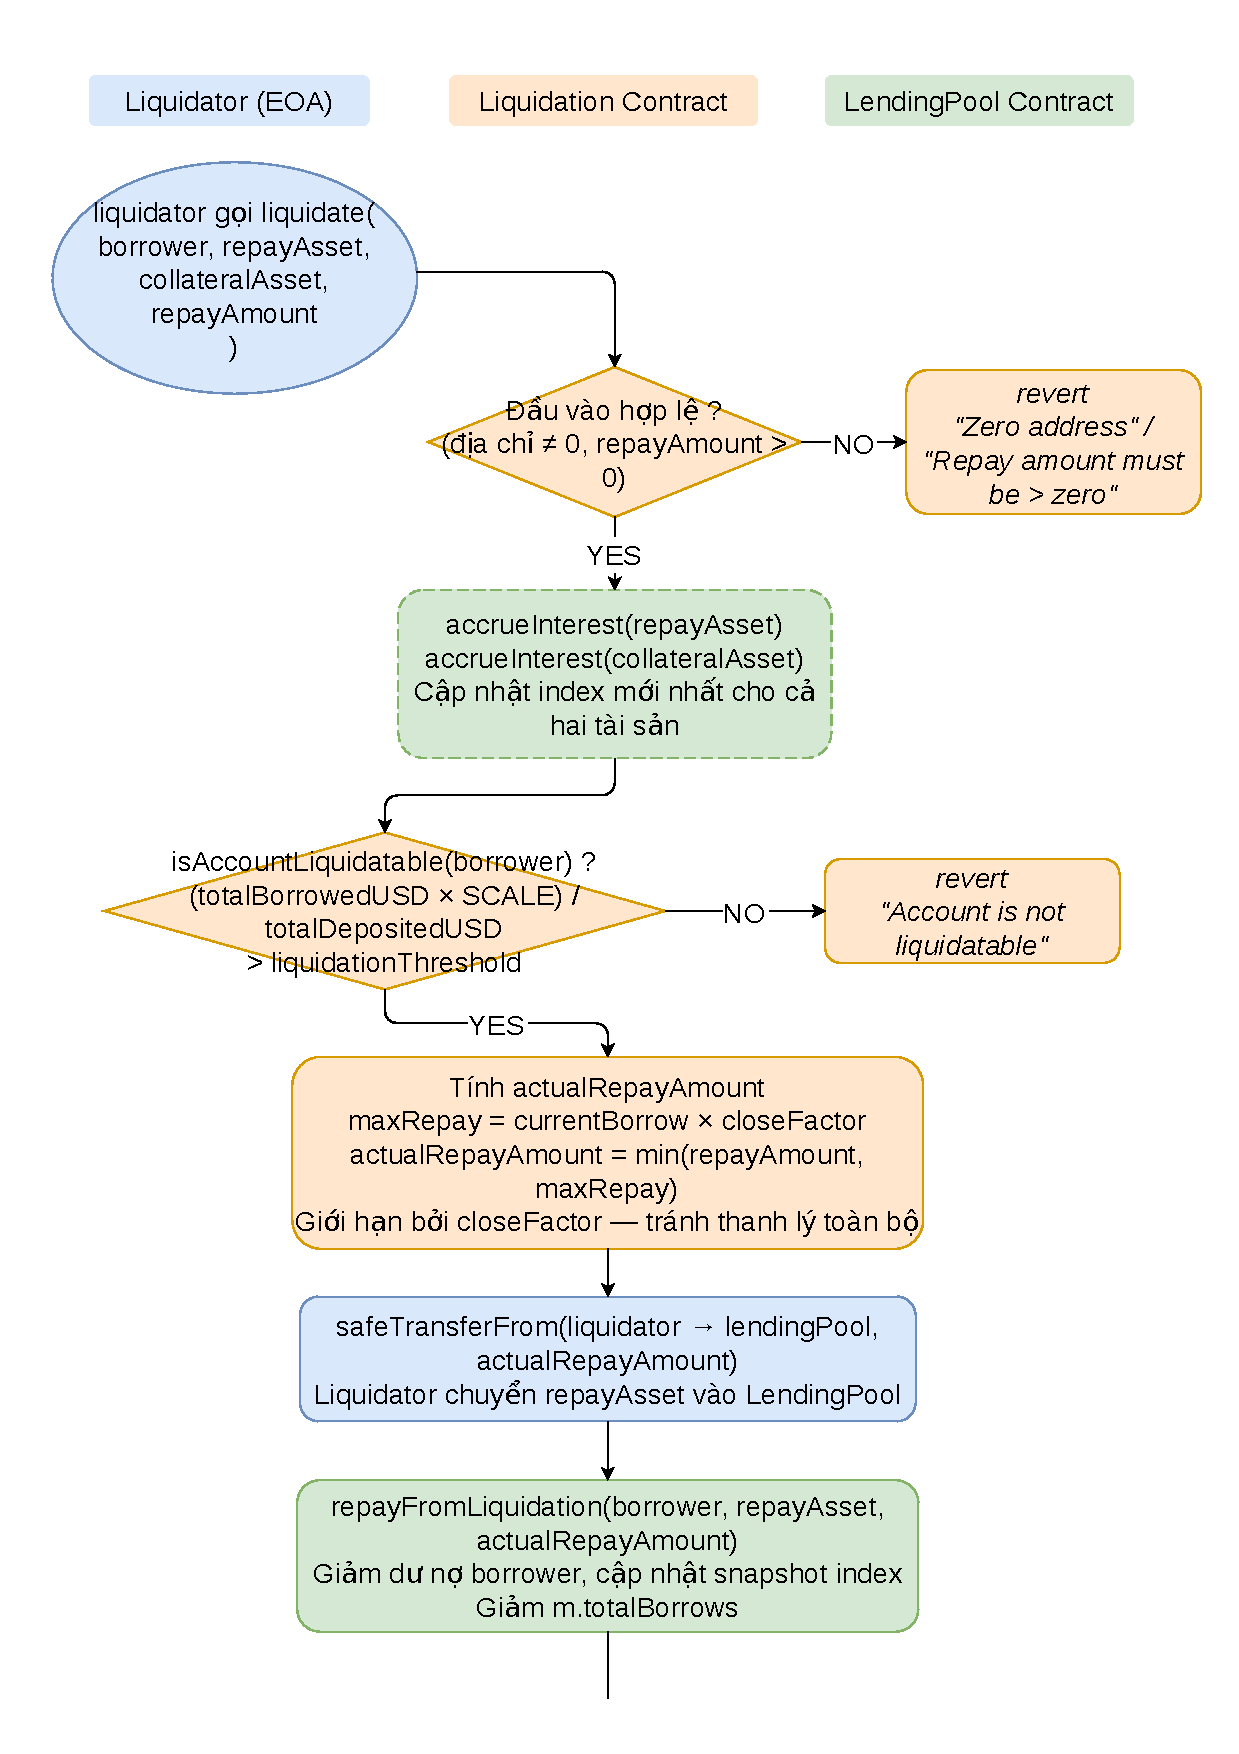
\includegraphics[
    page=1,
    width=\textwidth,
    height=0.51\textheight,
    keepaspectratio
]{../Hinhve/LF.pdf}

\includegraphics[
    page=2,
    width=\textwidth,
    height=0.51\textheight,
    keepaspectratio
]{../Hinhve/LF.pdf}

\caption{Sơ đồ luồng thanh lý}
\label{fig:lf}
\end{figure}



Công thức tính seize amount khi liquidate sử dụng liquidationIncentive, có ý nghĩa kinh tế khi Liquidator trả X USD tiền nợ, nhận lại X $\times$ (1 + incentive) USD tài sản thế chấp, đây là lợi nhuận của liquidator, đồng thời là động lực để duy trì sức khoẻ giao thức.

Giao thức xử lý cẩn thận trường hợp tài sản có số decimals khác nhau (ví dụ USDC = 6, WETH = 18), bằng cách chuẩn hóa tất cả về 18 decimals để tính toán rồi sau đó convert ngược về decimals gốc của tài sản khi trả kết quả.

\begin{align}
\mathrm{repayAmount}_{18} &= \mathrm{repayAmount} \times 10^{(18 - d_{\mathrm{repay}})} \quad \text{(chuẩn hóa lên 18 decimals)} \label{eq:repay_normalize} \\
\mathrm{seizeAmount}_{18} &= \mathrm{repayAmount}_{18} \times (1 + \mathrm{incentive}) \times \frac{p_{\mathrm{borrowed}}}{p_{\mathrm{collateral}}} \label{eq:seize_amount} \\
\mathrm{seizeAmount} &= \frac{\mathrm{seizeAmount}_{18}}{10^{(18 - d_{\mathrm{collateral}})}} \quad \text{(convert về collateral decimals)} \label{eq:seize_denormalize}
\end{align}


\subsection{PriceRouter / PriceRouterStorage}


Contract này đóng vai trò là một tầng Oracle Abstraction Layer, đóng vai trò trung gian giữa giao thức và nguồn giá, tất cả các smart contract cần giá tài sản (LendingPool, Liquidation) đều gọi qua PriceRouter.getPrice(), không bao giờ gọi trực tiếp oracle. Thiết kế này mang đến tính linh hoạt cho giao thức: Có thể thêm nguồn giá mới mà không cần sửa LendingPool/Liquidation, đồng thời PriceRouter cũng được cài đặt UUPS, có thể upgrade logic mà không đổi địa chỉ.

Mô hình dữ liệu của PriceRouter gồm có

\begin{lstlisting}
enum Source { CHAINLINK, MYORACLE, NONE }

struct FeedInfo {
  Source source;          // nguon gia
  address feedOrToken;    // Chainlink feed address hoac token address (cho MyOracle)
}

mapping(address => FeedInfo) feeds; // asset => nguon gia
__gap[47] // du tru storage slot cho UUPS upgrade, tong 50 slot (3 bien + 47 gap).
\end{lstlisting}


PriceRouter của giao thức được sử dụng để lưu trữ nguồn giá của một loại asset, sử dụng Chainlink hoặc nguồn giá từ MyOracle, trong môi trường Production, cần phải sử dụng Chainlink hoặc các dịch vụ Oracle on-chain tương tự.
\begin{lstlisting}
feeds[asset].source == NONE      -> revert "No price feed available"
feeds[asset].source == CHAINLINK -> goi AggregatorV3Interface.latestRoundData()
feeds[asset].source == MYORACLE  -> goi MyOracle.getPriceMyOracle(asset)
\end{lstlisting}

Đặc biệt, đối với Chainlink Feed, giao thức có cơ chế bảo vệ khi xảy ra Stale Price, giá on-chain bị chậm và không còn được cập nhật kịp thời, smart contract PriceRouter thực hiện 3 lớp validation đối với giá từ Chainlink:

\begin{lstlisting}
(
    uint80 roundId,
    int chainlinkPrice,
    ,
    uint updatedAt,
    uint80 answeredInRound
) = priceFeed.latestRoundData();

require(updatedAt > 0, "Round not complete");
require(answeredInRound >= roundId, "Stale price");
require(chainlinkPrice > 0, "Invalid price from Chainlink");
\end{lstlisting}

Mặc dù PriceRouter đã triển khai ba lớp kiểm tra cơ bản đối với giá từ Chainlink, giao thức hiện chưa xác minh khoảng thời gian tối đa kể từ lần cập nhật giá gần nhất (staleness timeout). Ba kiểm tra hiện có đảm bảo giá hợp lệ về mặt cấu trúc --- round hoàn tất, round không bị lỗi, giá dương --- nhưng không ngăn được trường hợp node Chainlink ngừng cập nhật trong nhiều giờ liên tiếp. Khi đó, giá cũ vẫn được chấp nhận, dẫn đến rủi ro định giá sai tài sản và có thể gây ra thanh lý không chính xác. Kiểm tra còn thiếu là: require(block.timestamp - updatedAt $\leq$ MAX\_STALENESS). Đây là giới hạn đã được nhận diện trong phạm vi đồ án; trong môi trường production, cần bổ sung tham số MAX\_STALENESS phù hợp với heartbeat của từng Chainlink feed, thường dao động từ 1 đến 24 giờ tùy loại tài sản theo tài liệu chính thức của Chainlink.

Cuối cùng, nguồn giá được quản lý bằng các hàm admin của giao thức (được biểu diễn trong bảng~\ref{table:price_feed_management}).

\begin{table}[H]
\centering
\resizebox{\textwidth}{!}{%
\begin{tabular}{|p{0.37\textwidth}|p{0.63\textwidth}|}
\hline
\textbf{Hàm} & \textbf{Mục đích} \\ \hline
setChainlinkFeed(asset, feed) & Gán Chainlink AggregatorV3 feed cho asset \\ \hline
setMyOracleFeed(asset) & Cài đặt asset dùng MyOracle \\ \hline
removeFeed(asset) & Xóa nguồn giá (asset sẽ không thể giao dịch) \\ \hline
\end{tabular}
}
\caption{Các hàm quản lý nguồn giá}
\label{table:price_feed_management}
\end{table}


\subsection{Lớp quản trị: ProtocolController + ProtocolTimelock}
\label{section:4.2.5}


Quản trị là điểm tập trung rủi ro lớn nhất trong một DeFi protocol: nếu quyền admin bị compromise, kẻ tấn công có thể thay đổi toàn bộ tham số, rút treasury, hoặc upgrade smart contract sang implementation độc hại trong một giao dịch duy nhất. Phân tích các rủi ro cụ thể của mô hình single admin và lý do lựa chọn kiến trúc quản trị 2 tầng (Multisig + Timelock) được trình bày tại mục~\ref{section:5.6}. Phần này mô tả thiết kế kỹ thuật của từng thành phần.

Toàn bộ giao thức được thiết kế theo kiến trúc quản trị 2 tầng, mọi hành động của admin, trước khi được thực thi đều phải đi qua Multisig Wallet và Timelock~\cite{SafeGlobalDocs,OpenZeppelinDocs}
\begin{lstlisting}
[Admin / Multisig Wallet]
  | proposal
[ProtocolTimelock]       <- ap dat do tre thoi gian (minDelay)
  | execute (sau minDelay)
[ProtocolController]     <- single entry point quan tri
  | goi
[LendingPool / Liquidation / PriceRouter / MyOracle]
\end{lstlisting}


\subsubsection{ProtocolController --- Single Entry Point Pattern}


ProtocolController là điểm vào duy nhất cho admin, kế thừa AccessControl của OpenZeppelin~\cite{OpenZeppelinDocs}. Các hàm quản trị hệ thống trong ProtocolController được biểu diễn trong bảng~\ref{table:admin_functions}.

\begin{table}[H]
\centering
\resizebox{\textwidth}{!}{%
\begin{tabular}{|p{0.21\textwidth}|p{0.45\textwidth}|p{0.34\textwidth}|}
\hline
\textbf{Nhóm} & \textbf{Ví dụ hàm} & \textbf{Tác động} \\ \hline
Quản lý địa chỉ smart contract & setLendingPool, setPriceRouter, setLiquidation & Cập nhật địa chỉ đồng bộ nhiều smart contract \\ \hline
Quản lý tài sản & supportMarket, unsupportMarket & Thêm/xóa tài sản khỏi giao thức \\ \hline
Cấu hình giá & setChainlinkFeed, setMyOracleFeed, setPrice & Quản lý nguồn giá tài sản \\ \hline
Cấu hình rủi ro & setCollateralParams, setLiquidateParams & Điều chỉnh tham số an toàn \\ \hline
Khẩn cấp & pauseLendingPool, unpauseLendingPool & Dừng/tiếp tục giao thức \\ \hline
Tài chính & withdrawTreasury, rescueToken & Quản lý ngân quỹ \\ \hline
Nâng cấp & upgradeLendingPool,  upgradePriceRouter & Nâng cấp UUPS implementation \\ \hline
Di chuyển & migrateController & Chuyển quyền điều khiển sang Controller mới \\ \hline
\end{tabular}
}
\caption{Các hàm quản trị admin}
\label{table:admin_functions}
\end{table}


ProtocolController có một cơ chế thiết kế đặc biệt, đó là Atomic Multi-Contract Update, cập nhật đồng thời nhiều smart contract cùng lúc, và đảm bảo tất cả đều được cập nhật giống nhau, ví dụ trong việc cập nhật địa chỉ smart contract PriceRouter:
\begin{lstlisting}
setPriceRouter(_priceRouter):
  -> ILiquidation.setPriceRouter(_priceRouter)  // 1 call
  -> ILendingPool.setPriceRouter(_priceRouter)  // 1 call
  -> priceRouter = _priceRouter                 // cap nhat local
\end{lstlisting}

Việc này đảm bảo không bao giờ có trạng thái "một smart contract dùng PriceRouter mới, smart contract kia vẫn dùng cũ". Nhiều hành động được đảm bảo thực hiện cùng nhau hoặc đều fail, ví dụ khi thêm một tài sản mới, đồng thời gọi supportMarket của LendingPool và setChainlinkFeed của PriceRouter:

\begin{lstlisting}
supportMarketWithChainlinkFeed(asset, irm, feed):
  -> LendingPool.supportMarket(asset, irm)      // them market
  -> PriceRouter.setChainlinkFeed(asset, feed)   // dang ky nguon gia
\end{lstlisting}


Đảm bảo này có căn cứ kỹ thuật từ tính nguyên tử (atomicity) của transaction trên Ethereum: toàn bộ các lệnh trong một transaction đều được thực thi hoặc đều bị revert cùng nhau, không có trạng thái trung gian nào được lưu lại trên blockchain nếu transaction thất bại. Do đó, nếu một lệnh cập nhật tại một smart contract nào đó revert vì bất kỳ lý do gì, toàn bộ transaction revert --- mọi smart contract đều giữ nguyên trạng thái cũ.

Quyết định thiết kế Atomic Multi-Contract Update và tầm quan trọng của nó trong bối cảnh quản trị phi tập trung được phân tích tại mục~\ref{section:5.6}.

\subsubsection{ProtocolTimelock}


Đây là một smart contract rất đặc biệt, smart contract này không thêm bất kỳ một logic mới nào, hoàn toàn kế thừa TimelockController của OpenZeppelin~\cite{OpenZeppelinDocs}:
\begin{lstlisting}
contract ProtocolTimelock is TimelockController {
  constructor(
    uint256 minDelay,
    address[] memory proposers,
    address[] memory executors,
    address admin
  ) TimelockController(minDelay, proposers, executors, admin) {}
}
\end{lstlisting}

Mục đích là để có địa chỉ smart contract riêng trên blockchain để track on-chain, đặt tên rõ ràng (ProtocolTimelock) để Etherscan verify và cộng đồng nhận biết, đồng thời cấu hình vai trò qua constructor: proposers (ai được đề xuất), executors (ai được thực thi). Khi deploy smart contract, timelock được cài đặt là admin của ProtocolController, tất cả các hàm của ProtocolController đều phải đi qua timelock. Luồng hoạt động của timelock rất đơn giản, dùng để chắc chắn không hành động nào của ProtocolController được thực thi ngay lập tức, mà phải chờ đợi qua minDelay:

\begin{lstlisting}
1. Proposer goi schedule(target, value, data, salt, delay) -> dang ky hanh dong cho
2. Cho minDelay (vi du: 48 gio)
3. Executor goi execute(target, value, data, predecessor, salt) -> thuc thi hanh dong
\end{lstlisting}


\section{Thiết kế cơ sở dữ liệu}


Cơ sở dữ liệu PostgreSQL được sử dụng với mục đích chính là để sao chép và tổ chức lại dữ liệu từ blockchain nhằm phục vụ truy vấn nhanh và hiển thị trên giao diện người dùng. Database không được xem là nguồn dữ liệu gốc (source of truth), toàn bộ dữ liệu đều có thể được tái tạo lại bằng cách replay lại các sự kiện đã phát sinh trên blockchain từ đầu. Hệ thống bao gồm tổng cộng 15 bảng, được chia thành 4 nhóm theo chức năng, sơ đồ ERD được thể hiện bởi hình~\ref{fig:ERD}.

\subsection{Nhóm 1: Dữ liệu nghiệp vụ giao thức (Protocol Business Data)}


Bảng assets lưu thông tin về các tài sản từng hỗ trợ trong giao thức. Mỗi tài sản được xác định duy nhất bởi cặp (assetAddress, chainId), cùng với ký hiệu (symbol), tên (name), số chữ số thập phân (decimals), trạng thái hỗ trợ hiện tại (isSupported), tổng số đã gửi (totalDeposited), tổng số đã vay (totalBorrowed), tổng số đã rút (totalWithdrawn), tổng số đã trả (totalRepaid), và số dư ngân quỹ giao thức (treasuryBalance). Số dư được lưu dạng DECIMAL(78,0) để đảm bảo không mất độ chính xác với số nguyên 256-bit của Solidity.

Bảng users lưu thông tin về các địa chỉ ví đã từng tương tác với giao thức, gồm địa chỉ ví (userAddress), mạng blockchain (chainId), email đăng ký nhận thông báo (nullable), và thời điểm lần đầu tham gia giao thức (joinedAt).

Bảng user\_assets lưu vị thế hiện tại của một người dùng đối với một tài sản cụ thể. Ngoài số dư đang gửi (depositedAmount) và số dư đang vay (borrowedAmount), bảng còn lưu lastSyncedBlock và lastSyncedLogIndex --- block và log index của lần quét cuối cùng --- để đảm bảo indexer có thể xử lý lại đúng thứ tự khi khởi động lại.

Bảng transactions lưu lịch sử toàn bộ giao dịch đã thực hiện trong giao thức. Mỗi bản ghi gồm hash giao dịch (duy nhất), người thực hiện (userId), tài sản liên quan (assetId), loại giao dịch (type: DEPOSIT/BORROW/REPAY/WITHDRAW/LIQUIDATE), số lượng token (amount), giá trị quy đổi USD tại thời điểm thực hiện (amountUSD) và số block (blockNumber).

Bảng asset\_configs lưu lịch sử thay đổi tham số cấu hình giao thức cho từng tài sản. Mỗi bản ghi ghi lại đầy đủ 9 tham số tại một thời điểm: 5 tham số mô hình lãi suất (baseRate, slope1, slope2, optimalUtilization, reserveFactor) và 4 tham số rủi ro (collateralFactor, closeFactor, liquidationIncentive, liquidationThreshold). Khi admin thay đổi bất kỳ tham số nào, một bản ghi mới được tạo ra thay vì cập nhật bản ghi cũ, nhờ đó cho phép truy vết lịch sử cấu hình đầy đủ.

\subsection{Nhóm 2: Dữ liệu log và snapshot (Historical \& Time-series Data)}


Bảng accrue\_logs lưu chi tiết mỗi lần tích lũy lãi suất (event Accrue từ smart contract). Mỗi bản ghi gồm tài sản liên quan (assetId), hash giao dịch, số block, tổng lãi đã tích lũy (interestAccrued), phần lãi chia cho người gửi (toDepositors), phần lãi vào treasury (toTreasury), và giá trị mới của tất cả các chỉ số quan trọng (newTotalBorrows, newBorrowIndex, newTotalDeposits, newDepositIndex). Bảng này cho phép backend tái tạo lại toàn bộ lịch sử lãi suất và phục vụ hiển thị biểu đồ biến động lãi theo thời gian.

Bảng treasury\_logs lưu lịch sử các thay đổi số dư ngân quỹ giao thức, bao gồm các sự kiện rút tiền (TreasuryWithdrawn) và donate vào ngân quỹ (Donated). Mỗi bản ghi ghi lại loại sự kiện (eventType), số lượng (amount), số dư sau thay đổi (balanceAfter), địa chỉ nguồn (fromAddress) và địa chỉ đích (toAddress).

Bảng asset\_snapshots lưu trạng thái tổng hợp của từng tài sản tại một block cụ thể, được tạo ra hằng ngày bởi tác vụ cron. Mỗi bản ghi ghi lại totalDeposited, totalBorrowed, treasuryBalance, utilizationRate, depositRate và borrowRate tại thời điểm snapshot. Dữ liệu này phục vụ hiển thị biểu đồ TVL (Total Value Locked) và lịch sử lãi suất trên giao diện người dùng.

Bảng user\_snapshots lưu trạng thái tổng hợp của từng người dùng tại một block cụ thể, cũng được tạo ra hằng ngày. Mỗi bản ghi ghi lại tổng giá trị đang gửi (totalDepositedUSD), tổng giá trị đang vay (totalBorrowedUSD), giá trị ròng (netWorthUSD) và hệ số sức khoẻ (healthFactor) của vị thế người dùng tại thời điểm đó.

\subsection{Nhóm 3: Dữ liệu quản trị (Governance Data)}


Bảng proposals lưu thông tin về các đề xuất quản trị được tạo thông qua Safe Multisig và Timelock. Mỗi proposal ghi lại địa chỉ smart contract mục tiêu (target), dữ liệu hàm được gọi ở dạng raw hex (calldata), trạng thái xử lý (status: 0-proposed / 1-scheduled / 2-executed / 3-cancelled), số chữ ký hiện tại (currentSigners), ngưỡng chữ ký cần thiết (multisigThreshold), hash giao dịch Safe (safeTxHash), hash giao dịch timelock (timelockExecutedTxHash), thời điểm có thể thực thi (eta) và ID thao tác trên Timelock (operationId). Đặc biệt, trường decodedAction lưu JSON đã được giải mã từ calldata, cho phép frontend hiển thị hành động admin một cách có thể đọc được thay vì hiển thị chuỗi hex thô.

\subsection{Nhóm 4: Dữ liệu hạ tầng hệ thống (Infrastructure State)}

Bảng scanners lưu trạng thái tiến độ quét blockchain theo từng mạng (chainId). Mỗi bản ghi chứa lastScannedBlock --- block cuối cùng đã xử lý thành công --- và lastScannedAt. Khi tiến trình indexer khởi động lại sau sự cố, nó đọc bảng này để biết phải tiếp tục từ đâu, đảm bảo không bỏ sót block nào.

Bảng cronner\_states lưu tiến trình snapshot hằng ngày của tác vụ cron. Mỗi bản ghi theo dõi loại snapshot (type: 0 = user snapshot, 1 = asset snapshot) và ID cuối cùng đã được snapshot (lastSnappedId). Cơ chế này cho phép tác vụ snapshot tiếp tục từ điểm dừng nếu bị gián đoạn giữa chừng, tránh phải xử lý lại từ đầu.

Bảng sessions lưu thông tin phiên đăng nhập của người dùng sau khi xác thực bằng chữ ký ví (SIWE). Mỗi session ghi lại token (duy nhất), thiết bị (device), địa chỉ IP (ip), người dùng sở hữu (createdById), thời điểm hết hạn (expired) và trạng thái thu hồi (revoked). Bảng hỗ trợ đa thiết bị --- một người dùng có thể có nhiều session hoạt động đồng thời trên các thiết bị khác nhau.

Bảng liquidatable\_users lưu danh sách các vị thế hiện đang đủ điều kiện bị thanh lý. Đây là bảng trạng thái động, được làm mới hoàn toàn mỗi 30 giây bởi tiến trình blc-indexer sau khi tính toán health factor của tất cả người dùng đang có nợ. Thông tin này được push real-time đến frontend qua WebSocket để hiển thị cảnh báo và hỗ trợ liquidator thực hiện thanh lý kịp thời.

\begin{figure}[H]
\centering
\includegraphics[width=0.9\textwidth]{Hinhve/ERD.png}
\includegraphics[width=0.9\textwidth]{Hinhve/ERD2.png}
\caption{Sơ đồ ERD của hệ thống}
\label{fig:ERD}
\end{figure}


\section{Thiết kế backend}


\subsection{Tổng quan kiến trúc --- Mô hình đa tiến trình Event-Driven}
\label{section:4.4.1}


Trước khi mô tả kiến trúc, cần nêu rõ bài toán mà kiến trúc này giải quyết. Hệ thống backend có 5 tác vụ với tính chất hoàn toàn khác nhau: quét blockchain liên tục, xử lý event bất đồng bộ, snapshot định kỳ, gửi thông báo, và phục vụ HTTP request. Nếu chạy chung một process, một tác vụ bị block hoặc crash sẽ kéo theo toàn bộ hệ thống.

Backend không được xây dựng theo mô hình monolith truyền thống mà theo kiến trúc đa tiến trình, hướng sự kiện (multi-process event-driven). Hệ thống gồm 5 worker độc lập, mỗi worker chạy trong một process riêng và giao tiếp với nhau qua RabbitMQ message queue~\cite{RabbitMQDocs} và Redis pub/sub. Không worker nào gọi trực tiếp vào tiến trình khác, toàn bộ phối hợp đều thông qua message. Cách các worker giao tiếp với nhau và với redis cùng message queue được trình bày bằng hình~\ref{fig:backend_architecture}.

Ưu điểm của kiến trúc này là mỗi tiến trình có thể được scale, khởi động lại hoặc nâng cấp độc lập mà không ảnh hưởng đến các tiến trình khác; kết hợp việc sử dụng RabbitMQ có khả năng hồi phục, đảm bảo không bị mất mát dữ liệu.

Phân tích lý do lựa chọn kiến trúc đa tiến trình thay vì monolith, cùng với lý do sử dụng RabbitMQ thay vì gọi trực tiếp, được trình bày tại mục~\ref{section:5.4}.

\begin{figure}[H]
\centering
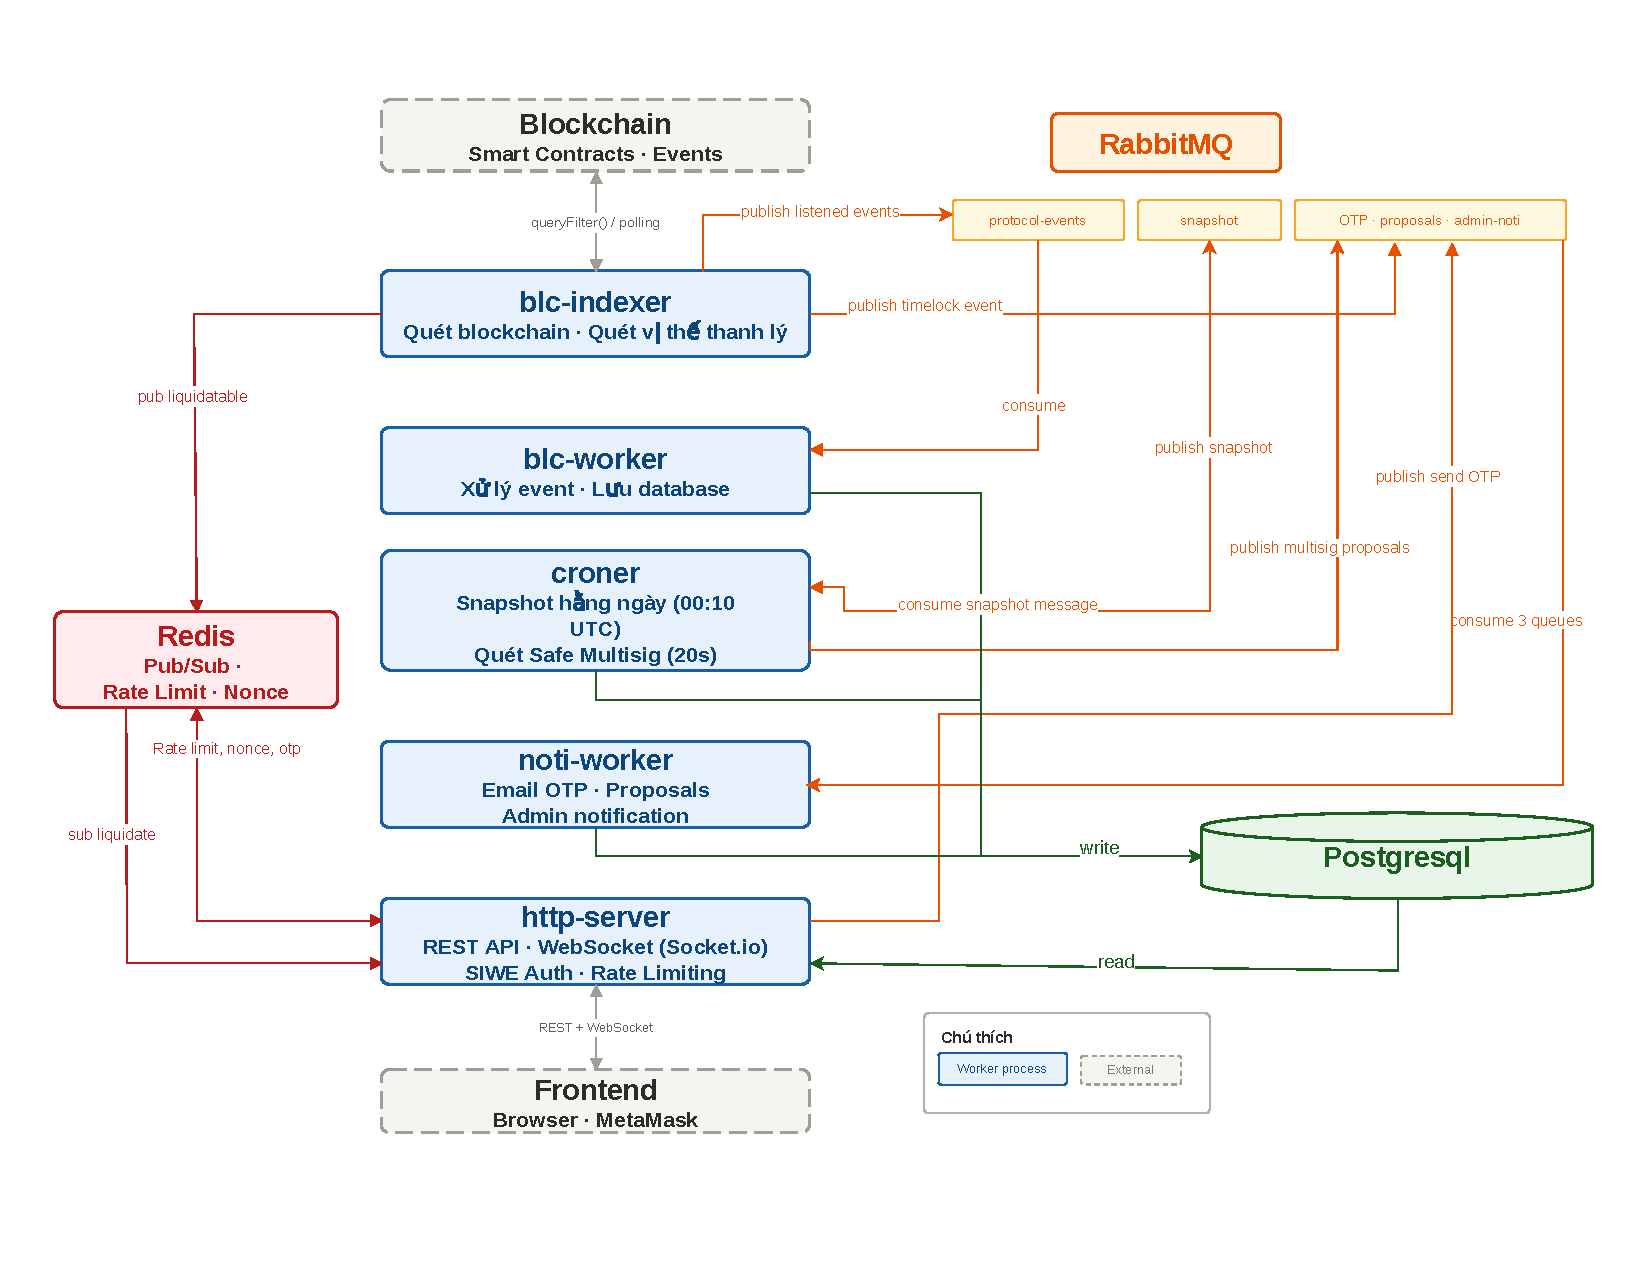
\includegraphics[
    page=1,
    width=\textwidth,
    height=0.9\textheight,
    keepaspectratio
]{../Hinhve/BEACTT.pdf}
\caption{Sơ đồ tổng quan hệ thống backend}
\label{fig:backend_architecture}
\end{figure}


\subsection{Blockchain indexer (blc-indexer)}


Đây là worker cốt lõi nhất của hệ thống backend, hoạt động như một "máy quét blockchain" liên tục, được cài đặt với mô hình mỗi chain tương ứng một cron job gọi scanChain() để xử lý các block mới của chain đó. Chu kỳ của cron job được cấu hình riêng theo block time của từng chain, ví dụ 12 giây với Ethereum Mainnet/Sepolia và 3,5 giây với BSC, tránh quét vô nghĩa khi chưa có block mới, đồng thời tạo nền tảng để mở rộng sang multi-chain mà không cần thay đổi logic lõi.

Trước khi mô tả luồng xử lý, cần biết trước một quyết định thiết kế nền tảng: indexer sử dụng mô hình polling (queryFilter) thay vì subscribe event theo thời gian thực. Phân tích chi tiết và so sánh hai hướng tiếp cận này được trình bày tại mục~\ref{section:5.5}. Ngắn gọn, lý do cốt lõi là polling cung cấp khả năng phục hồi trạng thái hoàn toàn sau downtime trong khi subscribe event không đảm bảo được tính chất này.

Luồng xử lý chính của scanChain() gồm 4 bước tuần tự:

Bước 1 --- Đọc điểm bắt đầu: Khi worker khởi động lần đầu, nếu bảng scanners chưa được khởi tạo cho chain đó, hệ thống đặt lastScannedBlock = currentBlock - 10 làm điểm xuất phát. Ở các lần chạy tiếp theo, worker truy vấn bảng scanners để lấy lastScannedBlock, từ đó tính fromBlock = lastScannedBlock + 1. Giới hạn trên toBlock được tính như sau:
\begin{lstlisting}
toBlock = min(currentBlock, fromBlock + MAX_BLOCK_RANGE - 1);
\end{lstlisting}


Giới hạn MAX\_BLOCK\_RANGE xử lý trường hợp worker bị downtime dài --- khi đó khoảng cách giữa fromBlock và currentBlock có thể lên đến hàng nghìn block, và quét toàn bộ một lần có thể vi phạm rate limit của nhà cung cấp RPC.

Bước 2 --- Quét events: Gọi đồng thời (Promise.all) 3 hàm quét trên cùng khoảng block \[fromBlock, toBlock\](i) scanLendingPoolContract quét toàn bộ event của LendingPool (Deposit, Borrow, Repay, Withdraw, Accrue, CollateralSeized, ...), (ii) scanLiquidationContract quét event thanh lý và (iii) scanTimelockContract quét event quản trị từ ProtocolTimelock (CallScheduled, CallExecuted, Cancelled), Mỗi hàm sử dụng \texttt{contract.queryFilter("*", fromBlock, toBlock)} để lấy toàn bộ event trong khoảng, sau đó sắp xếp theo blockNumber và logIndex tăng dần để đảm bảo xử lý đúng thứ tự thời gian.

Bước 3 --- Dispatch event: Mỗi event được tra cứu trong bảng protocolEventHandlers - một map từ tên event sang handler function tương ứng. Nếu tìm thấy handler, event được đẩy vào message queue RabbitMQ để blc-worker xử lý bất đồng bộ; nếu không tìm thấy, event bị bỏ qua và ghi log cảnh báo. Thiết kế tách biệt giữa việc indexer chỉ phát hiện và dispatch, worker mới xử lý nghiệp vụ.

Bước 4 --- Lưu block headers và cập nhật scanner: Toàn bộ thao tác ghi trong bước này được bao trong một Sequelize database transaction duy nhất: lưu block headers (number, hash, parentHash) vào bảng blocks và cập nhật lastScannedBlock trong bảng scanners. Tính atomicity đảm bảo không xảy ra trạng thái không nhất quán, hoặc cả hai thao tác đều thành công, hoặc đều rollback.

\subsection{Cơ chế quét và phát hiện vị thế thanh lý}


Mỗi 30 giây, blc-indexer chạy thêm một cron job để phát hiện các vị thế có thể bị thanh lý. Thuật toán sử dụng cursor-based pagination thay vì load toàn bộ người dùng vào bộ nhớ một lần --- an toàn khi số lượng người dùng lớn:

Bước 1: Truy vấn database theo từng batch 100 người dùng có borrowedAmount $>$ 0 (đang có nợ), sắp xếp theo userId tăng dần, dùng userId cuối của batch làm cursor cho lần tiếp theo.

Bước 2: Với mỗi địa chỉ ví trong batch, gọi isAccountLiquidatable(address) trực tiếp trên blockchain để kiểm tra health factor.

Bước 3: Nếu vị thế có thể bị thanh lý, upsert vào bảng liquidatable\_users. Nếu không còn đủ điều kiện, xóa khỏi bảng.

Bước 4: Sau khi quét xong toàn bộ, publish sự kiện LiquidatableUsersUpdated vào Redis pub/sub, kèm danh sách địa chỉ và block number hiện tại. HTTP server nhận event này qua Redis subscription và push ngay đến frontend qua WebSocket.

\subsection{Tiến trình Blockchain Worker (blc-worker)}


Tiến trình này lắng nghe queue RabbitMQ và xử lý các message do blc-indexer publish sau khi phát hiện event. Kiến trúc consumer–handler tách biệt hai trách nhiệm: BLCConsumerService chịu trách nhiệm lấy message từ queue và acknowledge; BLCWorkerHandler chịu trách nhiệm xử lý nghiệp vụ thực tế (parse event, lưu database).

Thiết kế này cho phép tăng số lượng blc-worker instance để xử lý song song khi lượng event lớn, mà không cần thay đổi blc-indexer.

\subsection{Tiến trình Cron (croner) và Snapshot hằng ngày}


Tiến trình croner đảm nhận 2 tác vụ định kỳ:

Snapshot hằng ngày (00:10 UTC): Tiến trình publish message vào RabbitMQ cho blc-worker xử lý --- snapshot trạng thái hiện tại của từng tài sản (lãi suất, TVL, utilization rate) và từng người dùng (totalDepositedUSD, totalBorrowedUSD, healthFactor) vào bảng asset\_snapshots và user\_snapshots. Trạng thái tiến độ được lưu vào bảng cronner\_states --- nếu bị gián đoạn giữa chừng, lần chạy tiếp theo tiếp tục từ ID cuối cùng đã snapshot thay vì chạy lại từ đầu.

Quét Safe Multisig (mỗi 20 giây): Gọi Safe API để lấy danh sách giao dịch đang chờ ký từ ví đa chữ ký của admin, cập nhật số chữ ký hiện tại và trạng thái vào bảng proposals. Nhờ đó, frontend có thể hiển thị lịch sử hành động admin một cách minh bạch mà không cần kết nối trực tiếp đến Safe API.

\subsection{Tiến trình Notification Worker (noti-worker)}


Tiến trình này lắng nghe đồng thời 3 loại message từ RabbitMQ:

Email consumer: Xử lý yêu cầu gửi email xác thực OTP khi người dùng đăng ký email nhận thông báo. Sử dụng Nodemailer với Email SMTP.

Proposal consumer: Nhận event về proposal mới từ blc-indexer, cập nhật trạng thái proposal vào database và thông báo cho admin.

Admin notification consumer: Theo dõi các thay đổi quan trọng của giao thức (thay đổi tham số, tạm dừng giao thức, thêm/xóa tài sản...) và gửi email thông báo đến tất cả người dùng đã đăng ký. Đây là lý do tại sao bảng users có trường email nullable --- chỉ người dung đã đăng ký mới nhận được thông báo.

\subsection{HTTP Server --- REST API và WebSocket}


HTTP server phục vụ frontend theo hai nhóm API có vai trò khác nhau. Nhóm thứ nhất là API dữ liệu giao thức (protocol data APIs), dùng để đọc dữ liệu mà backend đã index từ blockchain và xử lý như thông tin tài sản, lịch sử giao dịch, snapshot và proposal quản trị. Với nhóm này, blockchain vẫn là nguồn dữ liệu gốc duy nhất (source of truth), còn backend chỉ đóng vai trò lớp truy vấn và tăng tốc hiển thị; vì vậy các endpoint thuộc nhóm dữ liệu giao thức chỉ cung cấp thao tác đọc, không có endpoint tạo, sửa hay xóa trạng thái giao thức. Nhóm thứ hai là API hỗ trợ ngoài chuỗi (off-chain support APIs), phục vụ các nhu cầu hạ tầng của ứng dụng như xác thực SIWE, quản lý session, gửi/ kiểm tra OTP và đăng ký email nhận thông báo. Các API này có thể sử dụng POST vì chúng thao tác lên dữ liệu phụ trợ ngoài chuỗi (nonce, session, OTP, email registration), không làm thay đổi trạng thái tài chính của giao thức trên blockchain. Các nhóm endpoint chính của HTTP server được trình bày trong bảng~\ref{table:api_groups}.

\begin{table}[H]
\centering
\resizebox{\textwidth}{!}{%
\begin{tabular}{|p{0.23\textwidth}|p{0.24\textwidth}|p{0.52\textwidth}|}
\hline
\textbf{Nhóm} & \textbf{Prefix} & \textbf{Mô tả} \\ \hline
Tài sản & /api/assets & Danh sách tài sản, thông số thị trường \\ \hline
Giao dịch & /api/transactions & Lịch sử giao dịch, cần xác thực \\ \hline
Người dùng & /api/users & Vị thế cá nhân, cần xác thực \\ \hline
Snapshot & /api/snapshots & Dữ liệu lịch sử cho biểu đồ \\ \hline
Proposals & /api/proposals & Danh sách hành động admin \\ \hline
Logs & /api/logs & Lịch sử tích lũy lãi suất \\ \hline
Xác thực & /api/auth & SIWE, refresh/revoke session \\ \hline
Email & /api/email & Gửi OTP, xác thực OTP, đăng ký email \\ \hline
\end{tabular}
}
\caption{Các nhóm endpoint của hệ thống}
\label{table:api_groups}
\end{table}


Mỗi request HTTP đi qua một pipeline middleware theo thứ tự: (1) IP Rate Limiter kiểm tra số request/phút từ IP (Redis sliding window) $\rightarrow$ (2) CORS kiểm tra origin $\rightarrow$ (3) Auth Middleware (chỉ với endpoint yêu cầu xác thực) tra cứu session token trong database, xác nhận chưa hết hạn và chưa bị thu hồi $\rightarrow$ (4) Route Handler xử lý nghiệp vụ và trả response. Server áp dụng IP rate limiting toàn cục 60 request/phút/IP (sliding window, lưu trong Redis) để bảo vệ API. Endpoint OTP có rate limit riêng nghiêm ngặt hơn để chống brute force, cụ thể 60s 1 lần gửi OTP và tối đa 5 lần thử OTP.

Các endpoint thuộc nhóm dữ liệu giao thức (assets, snapshots, proposals, logs) không yêu cầu xác thực --- bất kỳ ai cũng có thể đọc dữ liệu công khai của giao thức. Các endpoint thuộc nhóm người dùng (transactions cá nhân, vị thế cá nhân) và off-chain support (email, session) yêu cầu token hợp lệ trong Authorization header.

WebSocket server (Socket.io) nhận event từ Redis pub/sub do blc-indexer publish và forward đến frontend đang kết nối --- kiến trúc hoàn toàn stateless, cho phép chạy nhiều instance HTTP server song song mà WebSocket vẫn hoạt động đúng nhờ Redis làm trung gian.


\end{document}
